% Formato para un capítulo cualquiera

%Título del capítulo
\chapter{Introducción} 
\label{sec:intro}
 
La estimación precisa de edades estelares es fundamentar para estudiar diferentes problemas astrofísicos. Por ejemplo, al buscar vida fuera del sistema solar, se sabe que el impacto de la vida en la atmósfera del exoplaneta anfitrión evoluciona con el tiempo, haciéndolo potencialmente detectable a través de biomarcadores. Por lo tanto, la datación de los exoplanetas detectados es fundamental y solo se puede realizar mediante la datación de su estrella anfitriona. En la arqueología galáctica, o en cómo la galaxia evoluciona con el tiempo, la datación de estrellas es la única forma de mapear esta evolución.

Entre todas las características estelares, la edad es la más dificil de obtener, ya que es la única que no se puede observar \emph{directamente} en nigún caso. Debe inferirse utilizandodiversos métodos. Soderblom presentó dos estudios que describen la mayoría de estas técnicas \cite{Soderblom15,Soderblom10}.

Dentro del grupo de enfoques para la datación estelar, una de las técnicas más prometedoras es la girocronología o datación de estrellas mediante su periodo de rotación. Las estrellas nacen con un rango de velocidades de rotación por diferentes razones físicas, ver \cite{Barnes03}. Entonces, el proceso llamado frenado magnético reduce la velocidad de rotación de la estrella con el tiempo \cite{Schatzman62}. Desde los finales de los 60's \cite{Belcher76,Kawaler88,Mestel68,Mestel87,Weber67}, se sabe que el frenado rotacional, o ley de frenado, es una función del periodo rotacional.
Es decir, cuanto mayor sea la rotación, mayor será el frenado. Por lo tanto, con el tiempo, todas las estrellas tienden a corverger a una velocidad de rotación similar para una edad y masa determinadas. Este efecto fue demostrado empíricamente por primera vez por Skumanich \cite{Skumanich72}. La girocronología es la técnica de datación estelar que explota este hecho \cite{Barnes16,Soderblom15}. Tradicionalmente, la girocronología se ha aplicado ajustando una expresión lineal que que contiene la edad estelar, su periodo de rotación y algunas aproximaciones de su masa. En trabajos recientes, Angus y otros \cite{Angus20,Angus19} han propuesto nuevas relaciones lineales clásicas para la girocronología combinadas con otras técnicas de datación, como el ajuste de isocronas o la cinemática estelar, en un marco bayesiano para una estimación de edad más precisa.

\section{Motivación}

Sin embargo, posiblemente, debido a la dificultad de recolectar muestras de datos que sean suficientes y precisas, no se ha intentado abordar el problema de la estimación de la edad de las estrellas como un ejercicio de regresión utilizando técnicas de inteligencia artificial. En este trabajo, se explora esta novedosa perspectiva, y las principales contribuciones son las siguientes.

En primer lugar, se ha recopilado un conjunto de datos para la girocronología. En general, el conocimiento aportado sobre la girocronología se basa principalmente en los cúmulos estelares, los únicos sistemas con una gran cantidad de estrellas con una determinación precisa de la edad. Para este trabajo se ha construido un muestreo completo y preciso con estrellas provenientes de cúmulos, pero también de astrosismología \cite{Angus15, Metcalfe19, Saders16}. La aparición de la astrosismología como una herramienta eficaz para datar estrellas ha permitido añadir una gran cantidad de estrellas de campo a la muestra. Todas las estrellas tienen una temperatura efectiva precisa ($T_{\rm eff}$), metalicidad ([Fe/H]), logaritmo de la gravedad superficial ($\log$ g), luminosidad ($L$), masa ($M$), radio ($R$), edad y periodo de rotación ($P_{\rm rot}$). La Sección \ref{sec:data} detalla la construcción de la muestra de datos, analizando fortalezas y debilidades. Supone un enfrentamiento cuando se quiere estimar las edades estelares utilizando la girocronología, principalmente porque aún no se comprende completamente la física y las dependencias físicas del fenómeno de frenado rotacional. Sin embargo, se cree que este es un problema interesante para que las técnicas de aprendizaje automático ofrezcan lo mejor de sí mismas.

En segundo lugar, se presenta pro primera vez un estudio comparativo de modelos de regresión de Inteligencia Artificial de última generación utilizando el conjunto de datos (consultar Sección \ref{sec:benchmarking}). Se incluye en el análisis un conjunto heterogéneo y completo de enfoques, que cubren: kNN clásico y regresión lineal o bayesiana; modelos combinados (bosque aleatorio, staking); preceso gaussiano; y redes neuronales. Se proponen hasta tres benchmarks diferentes, donde se comparan todos estos modelos para entender si precisión, robustez y capacidad de generalización.

Finalmente, en la Sección \ref{sec:results}, se revelan los resultados de los experimentos llevados a cabo, donde algunos modelos logran un MAE de $<0.5$ Gyr en estimación de edades estelares, lo que puede considerarse un avance significativo en el campo. Además, para fomentar una mayor investigación sobre el problema, se publica la muestra de datos, los códigos para reproducir los experimentos y todos los protocolos de evaluación diseñados. 

 

\chapter{Trabajos relacionados} 
\label{sec:related_work}

\section{Girocronología}
El beneficio principal de la girocronología está relacionado con la facilidad para obtener las entradas de observación requeridas: proxies fotométricos o espectroscópicos de la masa estellar y el periodo de rotación. Por otro lado, presenta una serie de incertidumbres que la convierten en una técnica de datación poco precisa, además de tener un rango de aplicación relativamente estrecho en términos de masa. En \cite{Barnes03} y \cite{Barnes07}, se publica por primera vez una ecuación empírica que permite estimar la edad estelar en función de su periodo de rotación y su índice de color. Esto puede considerarse como el origen de la girocronología como técnica prática. Esta relación empírica ha sido revisada posteriormente, en \cite{MH}, \cite{Barnes10} y \cite{Angus15}, utilizando una muestra de datos astrosísmicos en la última de estas. Pero en la vida real no suele ser tan sencilla. El frenado rotacional está ligado a la existencia de un campo magnético estelar bipolar. El mejor candidato para la dínamo que genera este campo es una zona convectiva exterior bien desarrollada.

Por lo tanto, solo las estrellas con masas inferiores al límite de Kraft \cite{Kraft67}, alrededor de 1,3 M, pueden reducir su velocidad de rotación con el tiempo siguiendo las leyes de ruptura conocidas. Pero, \cite{Zorec12} mostró que las estrellas A también tienen velocidades de rotación que evolucionan con el tiempo, esto puede deberse a que en estas estrellas también pueden encontrarse fuertes campos magnéticos, o al menos sus firmas \cite{Balona17}, y por lo tanto, por encima del límite de Kraft, el frenado rotacional puede seguir existiendo. En este rango de masas, por encima de 1,3 M, el mecanismo exacto de frenado es casi desconocido.

Para las estrellas jóvenes, la girocronología solo puede aplicarse a cúmulos de estrellas o grupos en movimiento \cite{Curtis19}. Para las estrellas individuales, la incertidumbre asociada solo permite una declaración general sobre si es o no es joven. Por otro lado, \cite{Saders16} encontro, comparando un conjunto de 21 estrellas fechadas usando astrosismología con modelos de frenado rotacional \cite{Saders13}, que a partir de cierto valor del número de Rossby, el frenado rotacional parece detenerse y la velocidad rotacional permanece en un estado estacionario, lo que hace que la girocronología tradicional sea casi inutil. En cualquier caso, este cambio en el régimen del frenado rotacionacional aún está en debate, con trabajos que lo confirman \cite{Gordon21}, \cite{Kitchatinov17}, \cite{Metcalfe19}, \cite{Metcalfe17} y \cite{Saders19}, y algunos otros que concluyen que no se observa, especialmente en el caso de gemelos solares en términos de masa y metalicidad \cite{Barnes16} y \cite{Oliveira19}.


\section{Modelos de IA para datación estelar}
Se pueden encontrar pocos trabajos que aborden el problema de la estimación de edades estelares mediante inteligencia artificial \cite{stardate}, \cite{Angus19}, \cite{das2018} y \cite{sanders2018}. Sander y Das presentan en \cite{sanders2018} un catálogo con distancias, masas y edades de 3 millones de estrellas se la segunda publicación de datos de Gaia. Las edades se estiman siguiendo un ajuste bayesiano a la estructura estelar y modelos de evolución, para caracterizar sus funciones de densidad de probabilidad. Angus y otros \cite{stardate}, \cite{Angus19} proponen una combinación de las relaciones lineales para girocronología con isócronas ajustadas bajo un marco de estimación bayesiano. Su enfoque utiliza un proceso de cadena de Markov Monte Carlo para inferir las edades. Es en \cite{sanders2018} donde encontramos por primera vez una Red Neuronal Bayesiana aplicada al problema de estimación de la edad. Técnicamente, Sander y Das entrenan un perceptrón multicapa, con una sola capa oculta de 10 neuronas, para generar distribuciones posteriores predictivas para la masa, edad y distancia de las estrellas. De esta manera, su modelo puede reemplazar la dependencia de la técnica de las isócronas. Las diferencias de todas estas obras con las nuestras son las siguientes. Todos los modelos anteriores abordan el problema desde una perspectiva bayesiana, centrándose en las predicciones de distribuciones posteriores de las edades. En cambio, aquí se propone un problema de regresión puro, donde los modelos se enfrentan a la estimación de un valor particular para la edad y se evalúan en consecuencia. Además, por este motivo, la comparación directa con estos trabajos anteriores no es tarea fácil.


\chapter{Base de datos}
\label{sec:data}

Se emplea una muestra de 1464 estrellas con edades precisas procedentes de la astrosismología o la pertenencia a un cúmulo. La muestra astreosísmica consta de 312 entradas para las cuales se han inferido observables estelares fundamentales precisos (temperatura efectiva, logaritmo de la gravedad superficial, masa, radio contenido estelar de hierro a hidrógeno) a partir de una combinación de observaciones fotométricas, espectrostópicas y astrosismología. La contribución más significativa proviene de \cite{Serenelli17}, con 224 entradas. Otras se obtuvieron de \cite{Ceillier16},\cite{Garcia14},\cite{Silva15} y \cite{Silva17}.

En términos de periodo de rotación, de las 312 entradas obtenidas de la astrosismología, se tomaron 293 periodos de \cite{Garcia14}. Los periodo restantes se tomaron de \cite{Ceillier16}, \cite{Mazeh15}, \cite{McQuillan13a}, \cite{McQuillan14}, \cite{Nielsen13} y \cite{Reinhold13}. García y otros. \cite{Garcia14} analizaron la tasa de rotación de la superficie en el subconjunto de estrellas de tipo solar Kepler estudiadas en \cite{Garcia14}. Los mismos métodos de análisis implementados en \cite{Garcia14} se adoptan en \cite{Ceillier16}. En \cite{Nielsen13}, por otro lado, Nielsen y otros calcularon un periodograma Lomb-Scargle (LS). Eligieron como periodo de rotación el valor mediano de todos los picos registrados de potencia máxima medidos en varios trimestres de los datos de Kepler. En \cite{Reinhold13} también se usa el periodograma LS, pero restringiendo el análisi exclusivamente a los datos de cadencia larga del tercer trimestre de Kepler.

Se complementa la muestra con estudios de clusters realizados por la misión Kepler/K2. Se recopilan un total de 1152 entradas tomadas de \cite{Barnes16}, \cite{Gonzalez16}, \cite{Meibom11}, \cite{Meibom15} y \cite{Rebull17}. En \cite{Barnes16} y \cite{Gonzalez16}, los autores estudiaron el antiguo cúmulo M67, analizando los datos de las curvas de luz Kepler/K2 Campaign 5. M67 es un objetivo interesante para la girocronología, ya que tiene aproximadamente la misma edad y comparte una composición química a la del Sol. M67 también es el grupo más antiguo de la muestra. Barner y otros \cite{Barnes16}, derivaron los periodos de rotación de superficie utilizando una combinación de cuatro métodos: minimización de la dispersión de fase, longitud mínima de la cuerda, método de detección de la señal del periodo bayesiano y función de autocorrelación. En \cite{Gonzalez16}, se utilizó el método de análisis de periodograma de Lomb-Scargle. La edad del cúmulo se estableció por \cite{Barnes16} y su concordancia con las edades derivadas de la cromosfera \cite{Giampapa06} y la isocrona \cite{Bellini10}. Meibom y otros en \cite{Meibom11} estudiaron NGC 6811 (ver \cite{Janes13}), y \cite{Meibom15}, reportaron periodos para estrellas en NGC 6819 (ver \cite{Jeffries13}). Estos dos grupos cierran la brecha de edad entre Praesepe y M67. Estos autores emplearon el método de periodograma LS para obtener los periodos de rotación. Además, para todos los periodos de rotación reportados, examinaron visualmente el periodograma y las curvas de luz, y también verificaron los periodos de forma independiente utilizando el algoritmo CLEAN. Se observó a Praesepe durante la Campaña 5 de Kepler/K2. En \cite{Rebull17}, los autores identificaron los periodos de rotación de superficie aplicando el periodograma Lomb-Scargle. Tomaron el periodo correspondiente al pico más fuerte del periodograma como periodo de rotación (con algunas excepciones). El estudio produjo periodos para más del 80\% de todas las curvas de luz de Praesepe. La estimación de la edad de este grupo ha sido objeto de cierto debate, con el valor más reciente establecido en $760 \pm 60$ Myr por \cite{Brandt15}.

Para trabajar con la mayor exactitud y precisión, se han completado la muestra de los clústeres con masas y radios derivados con un modelo de Random Forest de aprendizaje automático del paquete R empiricalRelationsMR \cite{Moya18}.

La muestra es, por lo tanto, una mezcla de cuatro clústeres con edades de 0.79, 1, 2.5 y 4.2 Gyrs que reúnen un total de 1152 estrellas, con masas y radios estimados mediante aprendizaje automático y datos empíricos. Por otro lado, se tienen 312 estrellas con masas, radios y edades determinadas mediante astrosismología y periodos de rotación precisos. Finalmente, se han seleccionado aquellas estrellas FGK y de secuencia principal con periodos de rotación inferiores a 50 días. La razón de este filtrado es que la física detrás de la girocronología ocurre principalmente en estos tipos estelares y, por lo tanto, está limitada a un rango de masas de 0.7 a 2. Además, los periodos de rotación superiores a 50 días difícilmente pueden explicarse por la estructura estelar actual y los modelos de evolución.

Se van a apartar 32 estrellas no agrupadas (incluido el Sol) datadas utilizando astrosismología con fines de prueba. Por lo tanto, se trabaja con una muestra final formada por 397 estrellas en clústeres más 240 estrellas estudiadas mediante astrosismología, es decir, un total de 637 estrellas.

Desafortunadamente, esta muestra exhibe dos sesgos importantes: 1) la muestra astrosísmica está sesgada hacia las estrellas masivas y viejas; y 2) la muestra basada en clústeres está cuantificada por edad y sesgada hacia edades más jóvenes. En los experimentos se muestra que, a pesar de los sesgos, las técnicas de aprendizaje automático pueden extraer información confiable del conjunto de datos para estimar edades estelares. Con el timepo, especialmente con las misiones espaciales actuales y futuras, estos sesgos se irán mitigando progresivamente, con la consecuente mejora de las estimaciones.


\section{Entendiendo la muestra}

En la Figura \ref{Fig:HR_select}, se muestra la posición en el diagrama HR de todas las estrellas MS seleccionadas. También se muestra cuáles son los miembros de un clúster y cuáles de han caracterizado mediante astrosismología. Aquí se puede ver que las estrellas astrosísmicas cubrenla zona más masiva y/o evolucionada del diagrama HR, y las estrellas del cúmulo son más jóvenes y también cubren la región de baja mas.

\begin{figure}[t]
\begin{center}
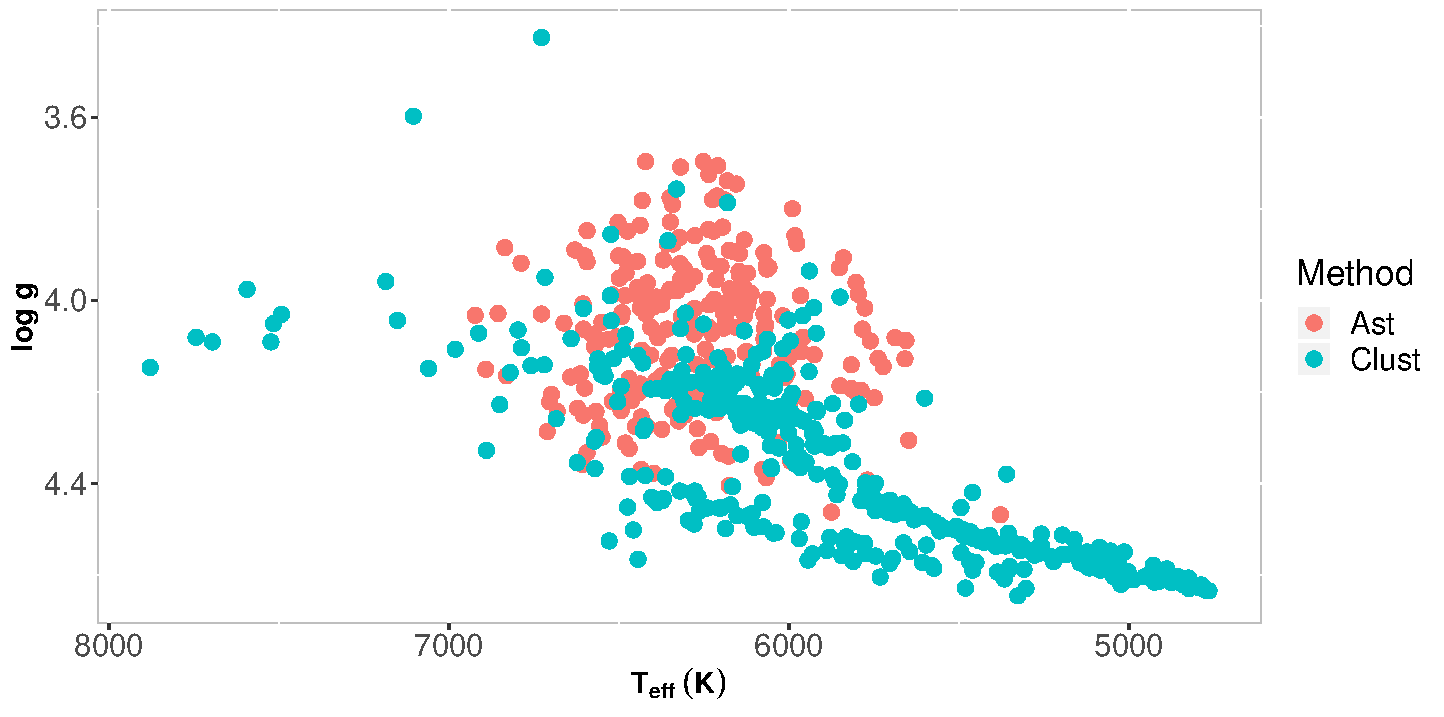
\includegraphics[width=0.9\linewidth]{Figuras/sampling_MS_astro_clust_embedded.pdf}
\end{center}
\caption{Diagrama HR mostrando la muestra MS.}
 \label{Fig:HR_select}
\end{figure}

\begin{figure}[t]
\begin{center}
 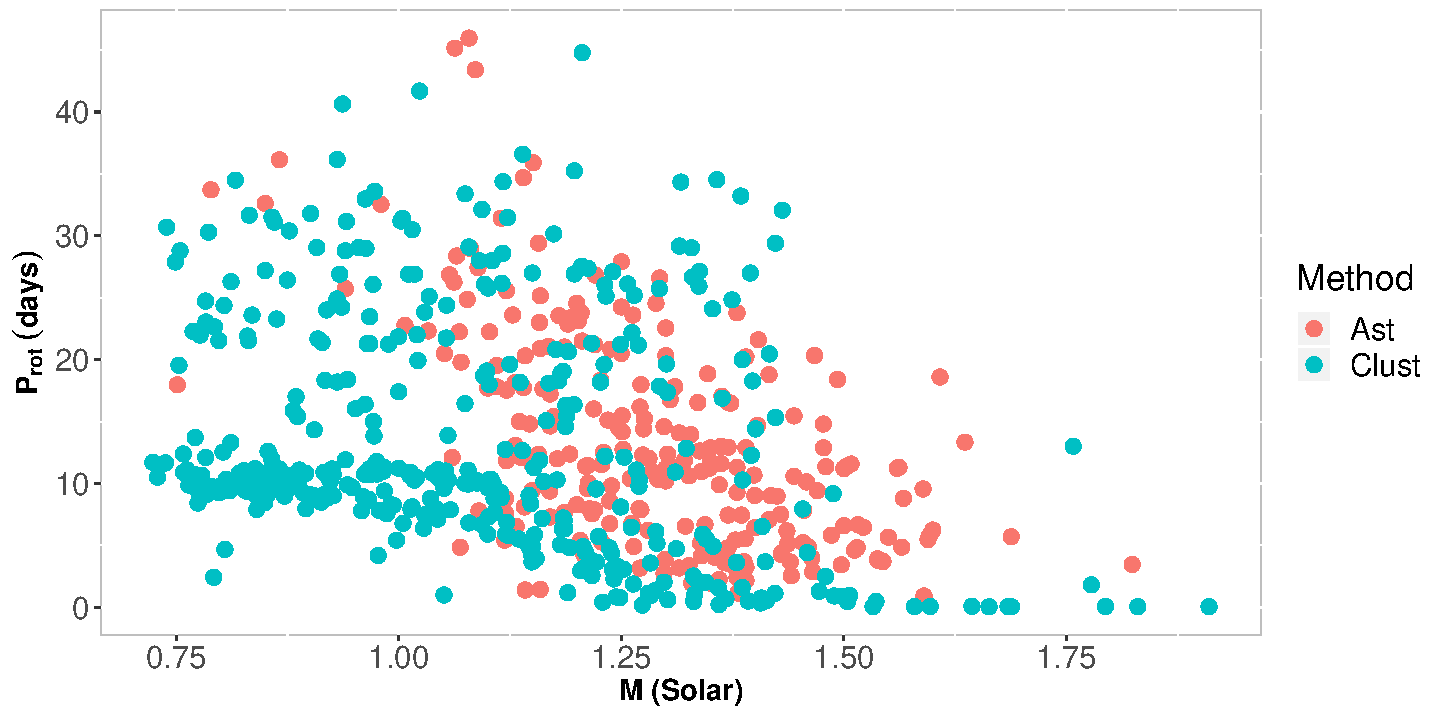
\includegraphics[width=0.9\linewidth]{Figuras/M_Prot_embedded.pdf}
\end{center}
\caption{$M$ - $P_{\rm rot}$ para las estrellas elegidas.}
 \label{Fig:M_rot}
\end{figure}

La idea clásica de la girocronología consiste en estimar las edades estelares utilizando cualquier indicador de la masa estelar y el periodo rotacional estelar. Como se tiene una estimación de masa para toda la muestra de entrenamiento, se puede representar directamente $M$ vs. $P_{\rm rot}$ (Fig. \ref{Fig:M_rot}), evitando usar esos indicadores. En este gráfico, también se diferencian las estrellas astrosísmicas de los cúmulos. No hay diferencias claras entre ellos, excepto el sesgo ya mencionado de la muestra astrosísmica hacia estrellas más masivas. El límite de Kraft está claro alrededor de 1,2M$_\odot$.


Si se añade la información de la edad estelar a la gráfica $M$ vs. $P_{\rm rot}$, se obtiene la Figura \ref{Fig:M_Age_rot}. Aquí se puede observar que, con una gran dispersión, cuanto mayor es $P_{\rm rot}$, mayor es la edad. Es destacable que también es cierto para estrellas masivas, por encima del límite de Kraft. Es decir, incluso en ausencia de una envolvente convectiva exterior desarrollada, también se produce la reducción de la velocidad de rotación con el tiempo.

\begin{figure}[t]
\begin{center}
 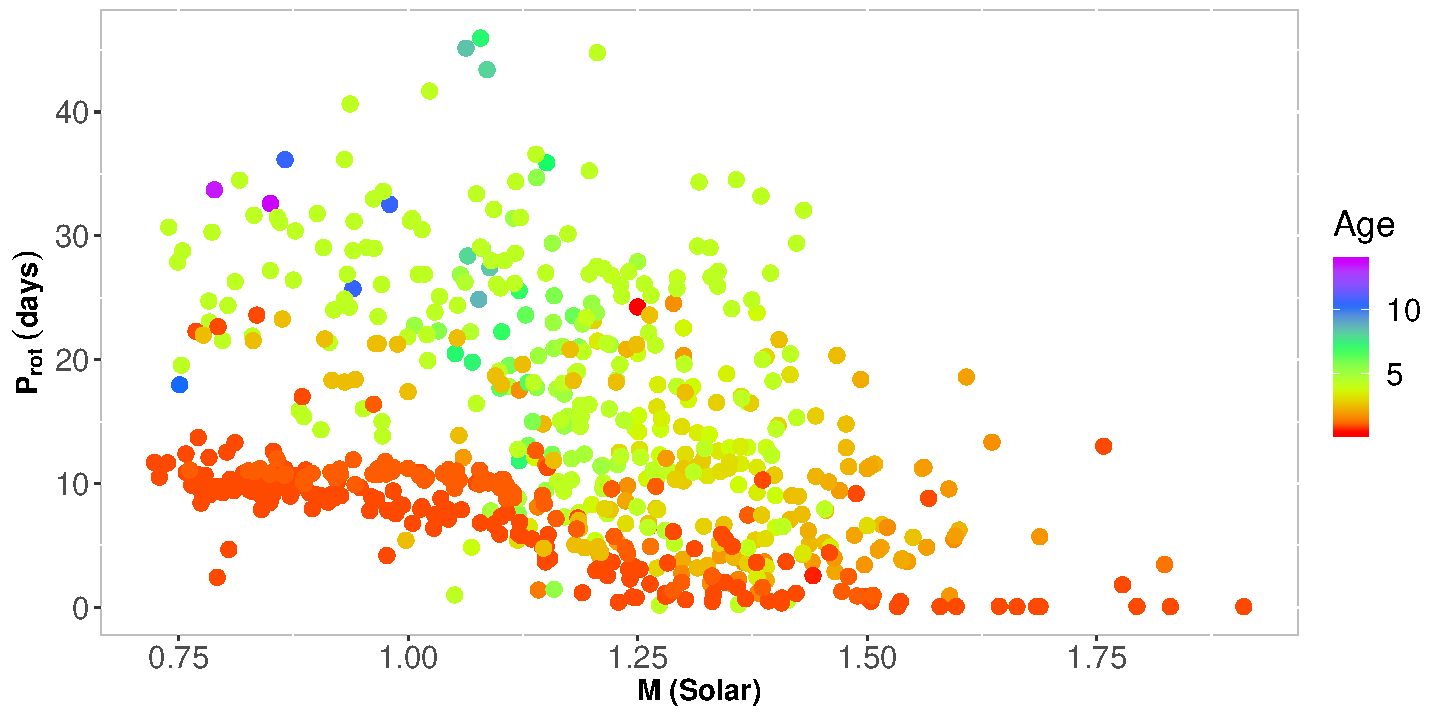
\includegraphics[width=0.8\linewidth]{Figuras/M_Prot_Age_embedded.pdf}
\end{center}
\caption{$M$ - $P_{\rm rot}$ para las estrellas elegidas. La edad se muestra en escala de color.}
 \label{Fig:M_Age_rot}
\end{figure}

\begin{figure}[t]
\begin{center}
 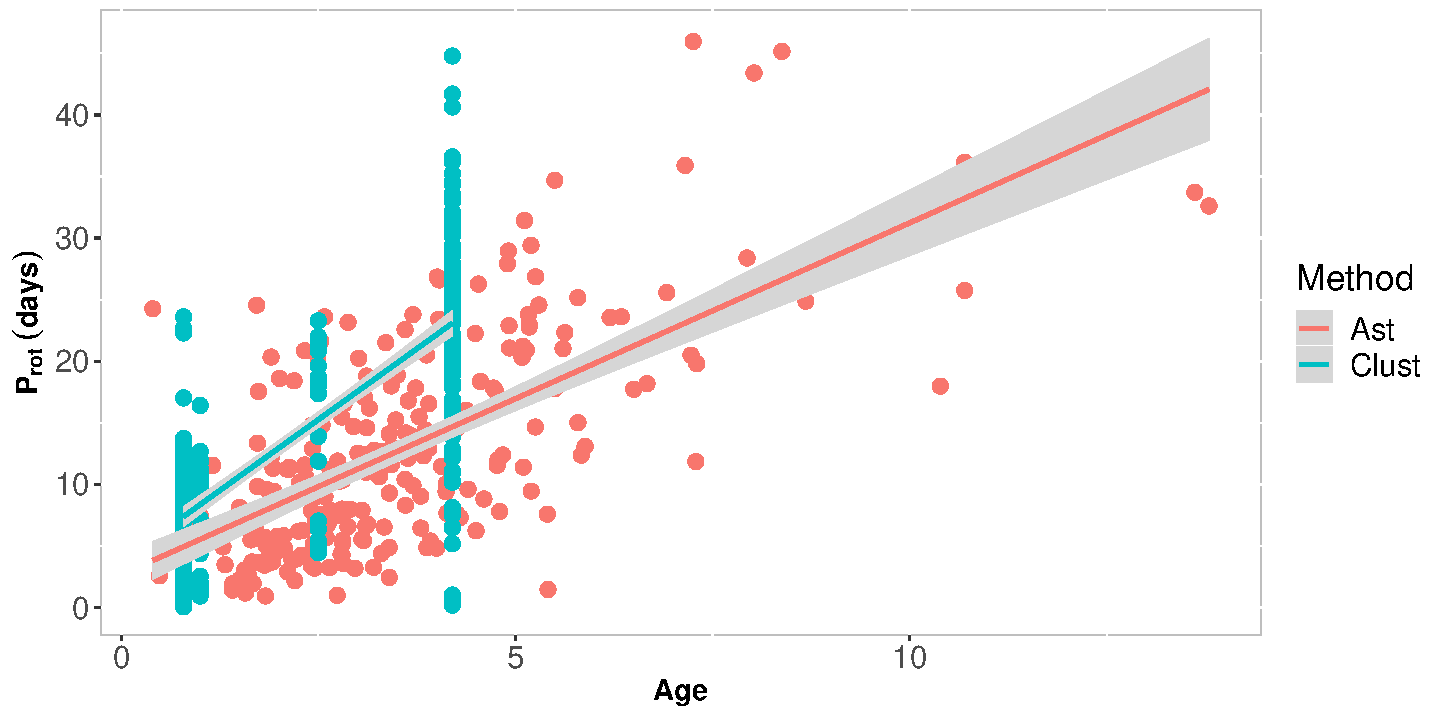
\includegraphics[width=0.8\linewidth]{Figuras/Age_Prot_embedded.pdf}
\end{center}
\caption{$Age$ - $P_{\rm rot}$ fpara las estrellas elegidas. Las estrellas asterosísimicas y de clúster se muestran en colores diferentes. También se representa la regresión lineal obtenida usando estos dos grupos.}
 \label{Fig:Age_rot}
\end{figure}

Si se representa la edad frente a su periodo de rotación, se obtiene la Figura \ref{Fig:Age_rot}. En general, se confirma que a mayor edad, mayor periodo de rotación, con una gran dispersión, principalmente para estrellas en cúmulos debido a la dependencia de masa del frenado de rotación. También se ha ajustado una regresión lineal a esta relación, diferenciando entre las estrellas astrosísmicas y los cúmulos. Aquí se puede observar uno de los sesgos de la muestra. Estas relaciones lineales tienen la misma tendencia pero apenas son diferentes para cada subgrupo. En cualquier caso, la dispersión es realmente grande y no se puede asegurar que estas regresiones se puedan utilizar para estimar la edad. Esta es la razón por la que se pasa a métodos de análisis basados en inteligencia artificial para generar modelos adecuados para estimaciones de edades estelares.


\chapter{Modelos y resultados} 

\section{Modelos}
\label{sec:models}

\textbf{Linear regressor} {} Primero se entrena un modelo de datación de estrellas asumiendo que la edad es combinación lineal de las características proporcionadas en la muestra de datos. Sea $\hat{a}$ el valor de la edad predecida, entonces
\begin{equation}
\hat{a}(\vb{w}, \vb{x}) = w_0 + w_1 x_1 + ... + w_D x_D \; ,
\end{equation}
donde $\vb{x}$ y $\vb{w}$ codifican el vector de características de entrada y el coeficiente del regresor lineal, respectivamente. Se sigue el enfoque de mínimos cuadrados para el aprendizaje del modelo, resolviendo un problema de forma: $\min_{\vb{w}} || \vb{X} \vb{w} - \vb{a}||_2^2$. $\vb{X}$. $\vb{X}$ es una matriz que contiene todos los vectores de entrenamiento y $\vb{a}$ es el vector de edades.

\textbf{Bayesian Regression} {} Se implementa un regresión Bayessian Ridge para estimar un modelo probabilístico del problema de datación estelar con la forma:

\begin{equation}
p(a|\vb{X},\vb{w},\alpha) = \mathcal{N}(a|\vb{X} \vb{w},\alpha)\; ,
\end{equation}

donde se asume la edad salida $a$ como una distribución gaussiana sobre $\vb{X}\vb{w}$. $\alpha$ se estima directamente a partir de los datos que se tratan como una variable aleatoria. E parámetro de regularización se ajusta a los datos disponibles, introduciendo sobre los hiperparámetros del modelo, \ie $\vb{w}$, el siguiente gaussiano esférico $p(\vb{w}|\lambda) =
\mathcal{N}(\vb{w}|0,\lambda^{-1}\mathbf{I}_{D})$.

\textbf{Decision Tree Regressor} {} Se usa un modelo de árbol de decisión \cite{Breiman1984}. Durante el aprendizaje, el modelo optimiza sus hiperparámetros internos a través de un proceso de grid search con validación cruzada. Especificamente, se ajustan: la estrategia par elegir la división en cada nodo del árbol (mejor o aleatorio); el número mínimo de muestras requeridas para estar en un nodo hoja (5, 10, 50, 100); y la función para medir la calidad de la división (error cuadrático medio, error cuadrático medio con la puntuación de mejora de Friedman para posibles divisiones, error absoluto medio reducción de la desviación de Poisson para encontrar divisiones). 

\textbf{Random Forest Regressor} {} Este modelo de regresión se implementa siguiendo el trabajo de Breiman \cite{Breiman2001}, donde los árboles de decisión se contruyen a partir de muestras de datos extraídas con reemplazo del conjunto de entrenamiento. De nuevo se usa un proceso de grid search más validación cruzada para ajustar los siguientes hiperparámetros: número de árboles (5, 10, 50, 100); número mínimo de muestras requeridas para estar en un nodo hoja (5, 10, 50, 100); y la función para medir la calidad de la división (error cuadrático medio o error medio absoluto).

\textbf{Support Vector Regression} {} En el estudio se incluye este modelo de regresión, basado en la implementación LibSVM para regresión, \cite{LIBSVM}, siguiendo la aproximación $\epsilon$-SVR. Se emplea el kernel RBF, y se realiza una un grid search con validación cruzada para ajustar el parámetro $C$ (1, 10, 100, 1000).

\textbf{Gaussian Process} {} Se entrena un regresor de proceso gaussiano \cite{Rasmussen2006}, donde se supone que la media anerior es constante y cero. Para la covarianza del anterior se usa un kernel que es la suma de los siguientes tres kernels. RBF, $k(\vb{x}_i, \vb{x}_j) = \text{exp}\left(- \frac{d(\vb{x}_i, \vb{x}_j)^2}{2l^2} \right)$, where $d(\cdot, \cdot)$ es la distancia euclídea y $l$ es el parámetro de escala de longitud. Producto escalar, $k(\vb{x}_i, \vb{x}_j) = \sigma_0 ^ 2 + \vb{x}_i \cdot \vb{x}_j$. Es un kernel no estacionario que se obtiene de la regresión lineal poniendo a priori los coeficiones de $x_i (i = 1, \ldots, N)$ y  $N(0, \sigma_0^2)$ para el sesgo. Y finalmente, White kernel, $k(x_i, x_j) = noise\_level \text{ if } x_i == x_j \text{ else } 0$. La aplicación clave del White kernel es parte de un kernel suma, donde describe la componente de ruido de la entrada. Ajustar su parámetro se corresponde con estimar el nivel de ruido en ese momento.

\textbf{kNN} {} También se incluye en la comparativa un regresor kNN. Básicamente, se ajusta el parámetro k (1, 5, 10, 15, 20, 50) y el tipo de función de ponderación que se usa para escalar la contribución de cada vecino. Se exploran dos tipos de funciones de ponderación: a) uniforme, donde todos los puntos en cada vecindario se ponderan por igual; y b) distancia, que pondera los puntos por la inversa de su distancia a un punto de consulta. 

\textbf{Neural Network} {} La arquitectura implementada se muestra en la figura \ref{fig:neural_network}. Esta consiste en un perceptrón multicapa. El modelo incluye una capa de entrada, un conjunto de 3 capas ocultas fully-connected con 50 unidades en cada una, y la capa de salida encargada de la regresión de las edades de las estrellas. Cada unidad oculta va seguida de una función de activación ReLU. Se usa como función de pérdida el error cuadrado,$Loss(\hat{a},a,W) = \frac{1}{2}||\hat{a} - a ||_2^2 + \frac{\alpha}{2} ||W||_2^2$, donde $W$ codifica los pesos de la red, y $\alpha$ es el parámetro de regularización. La retropropagación \cite{LeCun2012} se utiliza para el aprendizaje del modelo con el optimizador SDG~\cite{sgd}. Durante el aprendizaje, se fija $\alpha=0.01$, y se usa una política de tasa de aprendizaje adaptativa, comenzando con un valor $0.1$.

\begin{figure}[t]
\begin{center}
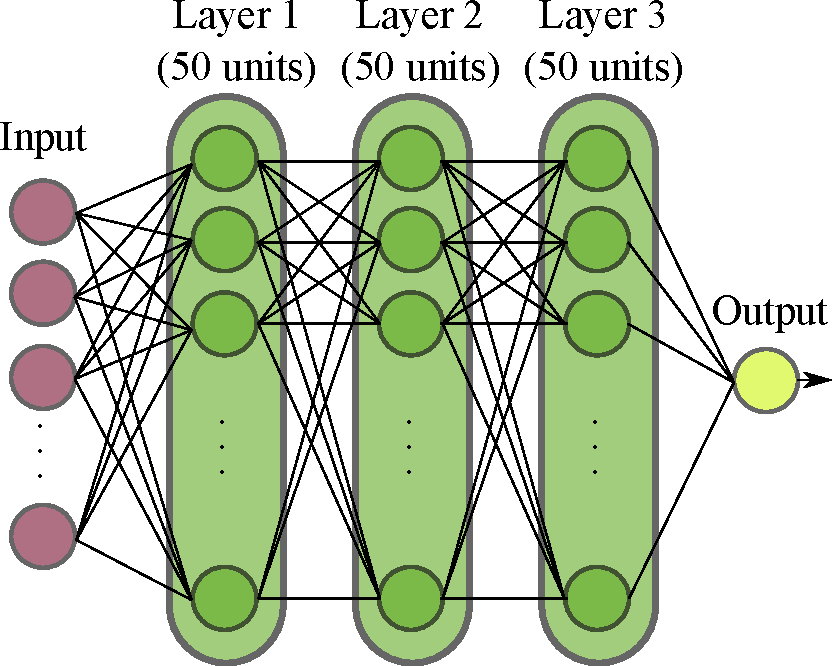
\includegraphics[width=0.6\linewidth]{Figuras/nnet.pdf}
\end{center}
\caption{Arquitectura de la red neuronal implementada. se han usado 3 capas ocultas, con 50 unidades en cada una seguida de una ReLU. La salida no tiene función de activación, para realizar directamente la estimación de la edad.}
\label{fig:neural_network}
\end{figure}

\textbf{Stacking} {} Finalmente, se emplea un método de ensamblado en machine learning conocido como generalización apilada o stacking \cite{Wolpert1992}. En un problema de regresión como lo es este, las predicciones de cada regresor individual (nivel 0) se apilan y se introducen en un estimador final (nivel 1), que calcula la predicción de la edad. Para este proyecto, en el nivel 0, se integran: neural network y Gaussian processes. Para la última capa (nivel 1), se incorpora un regresor lineal. Durante el entrenamiento, y para generalizar y evitar sobreajuste, el estimador de nievl 1 se entrena con muestras externas (tomadas del conjunto de entrenamiento), siguiendo una metodología de validación cruzada.

\section{Benchmark}
\label{sec:benchmark}

La muestra de datos, detallada en la Sección \ref{sec:data}, ofrece más de 600 estrellas, con edades precisas, donde se propone construir los siguientes escenarios de evaluación.

\textbf{Problema de datación estelar (Benchmark A)} {} En esta configuración, se propone evaluar los diferentes modelos de regresión siguiendo un esquema clásico de división de datos de entrenamiento/prueba. A partir de la distribución de la muestra de datos, se define un conjunto de entrenamiento y un conjunto de pruebas, donde el  80 \% y el 20 \% de las estrellas se han incluido al azar, respectivamente.

\textbf{Capacidad de generalización (Benchmark B)} {} En primer lugar, se proporciona un estudio de generalización para los modelos, donde se entrena con un enfoque de estrellas \emph{jóvenes}, y se evalúa su rendimiento en estrellas \emph{viejas}. Este escenario, denominado Benchmark B1, es interesante para evaluar la capacidad de los modelos de inteligencia artificial para trabajar con estrellas cuyo rango está fuera del conjunto de entrenamiento. Los rangos de edad de entrenamiento y prueba son $[0.4,4.2]$ y $[4.2,13.8]$ Gyr, respectivamente.

Se propone un segundo escenario para evaluar la capacidad de generalización de los modelos cuando se entrenan solo con estrellas pertenecientes a cúmulos. En la práctica, la girocronología se utiliza para datar estrellas individuales que pueden tener cualquier edad. Las estrellas de los cúmulos suelen estar datadas gracias a su pertenencia a los propios cúmulos. En este Benchmark B2, se propone el entrenamiento de los modelos utilizando únicamente estrellas pertenecientes a cúmulos. El resto de estrellas se incluyen en el conjunto de prueba. En total, este escenario recoge 397 y 240 muestras para entrenamiento y prueba, respectivamente.

\textbf{Regresión para datación estelar sobre una muestra de control (Benchmark C)} {} Aquí se propone examinar el rendimiento de todos los modelos sobre una muestra de datos de control compuesta por estrellas que no pertenecen a ningún cúmulo, y con una distribución más realista. Especificamente, en este Benchmark C, se evalúan los modelos entrenados con toda la muestra de datos sobre un conjunto de $32$ estrellas nuevas no pertenecientes a clústeres, incluyendo al Sol. Este conjunto independiente de control se ha obtenido de las mismas fuentes basadas en astrisismología utilizadas para recopilar la información de la muestra descrita en la Sección \ref{sec:data}. Se han reservado 32 estrellas de estas fuentes, antes de contruir la muestra. El rango de edad de este conjunto va de 1,2 a 10,1 Gyr. Este rango se superpone con el rango de edad utilizado en la muestra de entrenamiento ($[0.4, 13.8]$ Gyr), e incluye algunas edades nuevas no observadas. Se presta especial atención a la precisión de los modelos para la estimación de la edad del Sol (4.6 Gyr).


\section{Resultados}
\label{sec:results}
A contnuación, se presenta la configuración experimental y se informa de los resultados obtenidos en la evaluación de los modelos detallados en la Sección \ref{sec:models}. Este benchmarking se realiza a traves de los 3 escenarios descritos: el efecto de los diferentes modelos (Benchmark A); la capacidad de generalización (Benchmark B); y el rendimiento sobre una muestra de control (Benchmark C).

\subsection{Configuración experimental}

\paragraph{Implementación} 
Para poder comparar manzanas con manzanas, se han creado todos los modelos de regresión en Python, usando la librería scikit-learn \cite{scikit-learn}. Se utilizan las siguientes siglas para identificar los modelos implementados: Red Neuronal (nnet), Regresor Lineal (lr), Árbol de Decisión (dtr), Bosque Aleatorio (rf), Máquina de Vectores Soporte (svm), Regresión Bayeiana (bayes), k-Próximos Vecinos (kNN), Proceso Gaussiano (gp) y Stacking (stacking).

\paragraph{Métricas de evaluación}
La métrica de evaluación principal utilizada es el error medio absoluto, $MAE = \frac{\sum_{i=1}^{N}|a_i-\hat{a}_i|}{N}$, where $a_i$ and $\hat{a}_i$, donde $a_i$ y $\hat{a}_i$ son la edad proporcionada por el conjunto de datos y la edad estimada por un modelo de regresión, respectivamente. Dado que el conjunto de datos proporciona información sobre la precisión de la edad de cada estrella, en forma de límites de error, también se propone utilizar como métrica de evaluación de la precisión el porcentaje de predicciones de la edad de las estrellas que se encuentran dentro del intervalo de confianza proporcionado por el propio conjunto de datos.

\subsection{Benchmark A: Problema de datación estelar}

La Figura \ref{fig: benchA_models} muestra el rendimiento de todos los modelos, comparan su MAE correspondiente. En este escenario es interesante de observar que se tienen 2 modelos, más su stacking, que presentan los mejores resultado, estableciendo un margen un margen con respecto a los demás. Son la Red Neuronal y el Proceso Gaussiano. Su Stacking reduce ligeramente el mejor ,AE de la Red Neuronal de 0,405 a 0,400. Las Figuras  \ref{fig:benchA_details_stacking}--\ref{fig:benchA_details_rf} ofrecen un análisis detallado de las predicciones para los 5 métodos prinicipales para todas las muestras de prueba. Curiosamente, la mayoría de los modelos presentan dificultades en la estimación de la edad de las estrellas más viejas. También es relevante el resultado proporcionado por un modelo tan simple como un kNN, con un MAE de solo 0,53 Gyr. Una posible explicación es que la base de datos tiene muchos elementos concentrados en 2 valores de edad muy específicos, lo que permite que modelos como kNN hagan estimaciones muy precisas sobre las estrellas de prueba con estas edades. Este hecho se corrobora en la Tabla \ref{table:precisions}, donde se observa que la mejor precisión la logra el modelo kNN, seguido por la Red Neuronal. En general, a excepción de lr y bayes, todos los modelos ofrecen un MAE por debajo de 0,86 Gyr, lo que supone un gran avance en el campo de la datación estelar.

\begin{figure}[t]
\begin{center}
 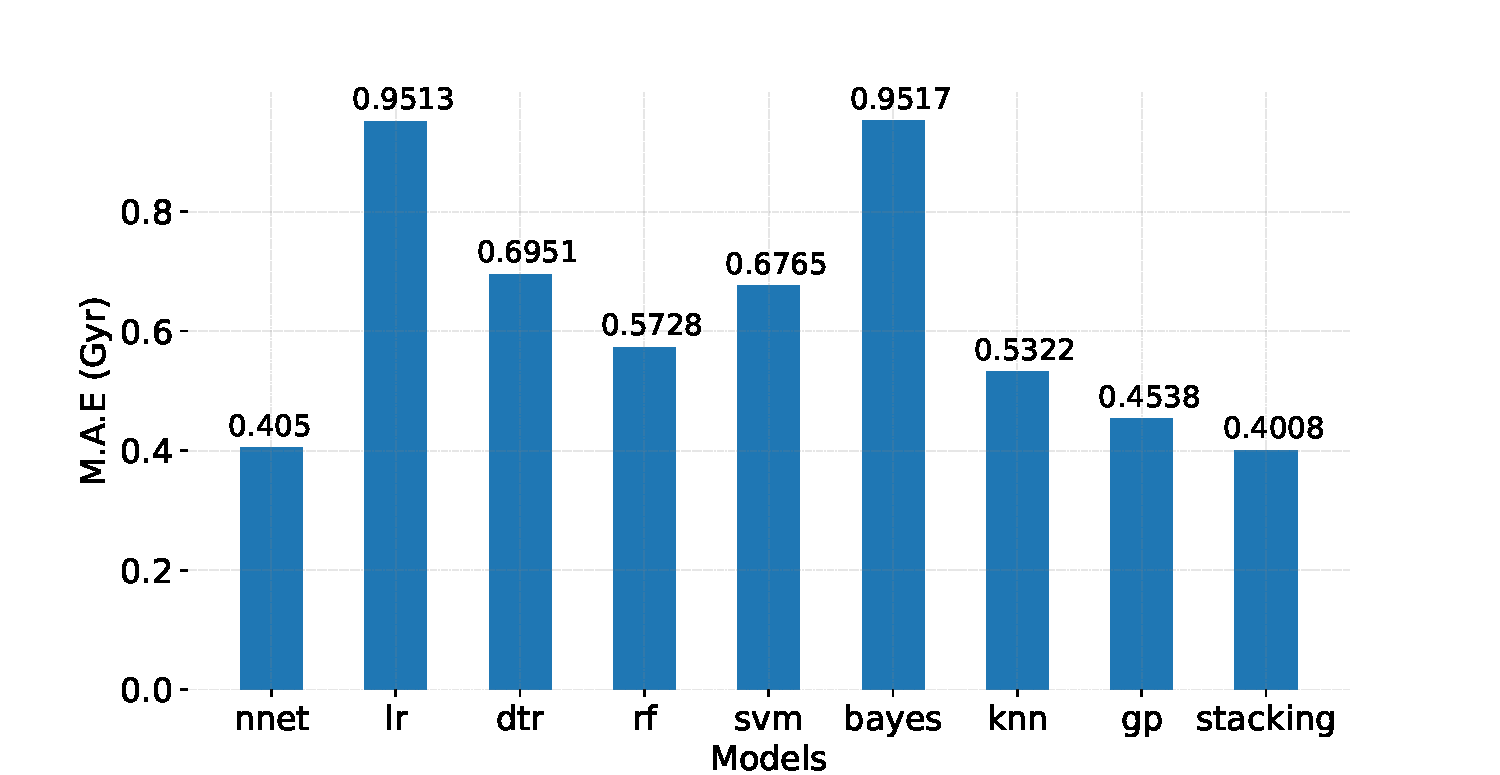
\includegraphics[width=0.8\linewidth]{Figuras/Experimentos/B_A_models.pdf}}
\end{center}
\caption{Rendimiento de los modelos en función del MAE. En esta configuración, las dos mejores aproximaciones son Neural Network (nnet) y Gaussian Process (gp), y por lo tanto, su stacking.}
 \label{fig:benchA_models}
\end{figure}

\begin{figure}[t]
\begin{center}
 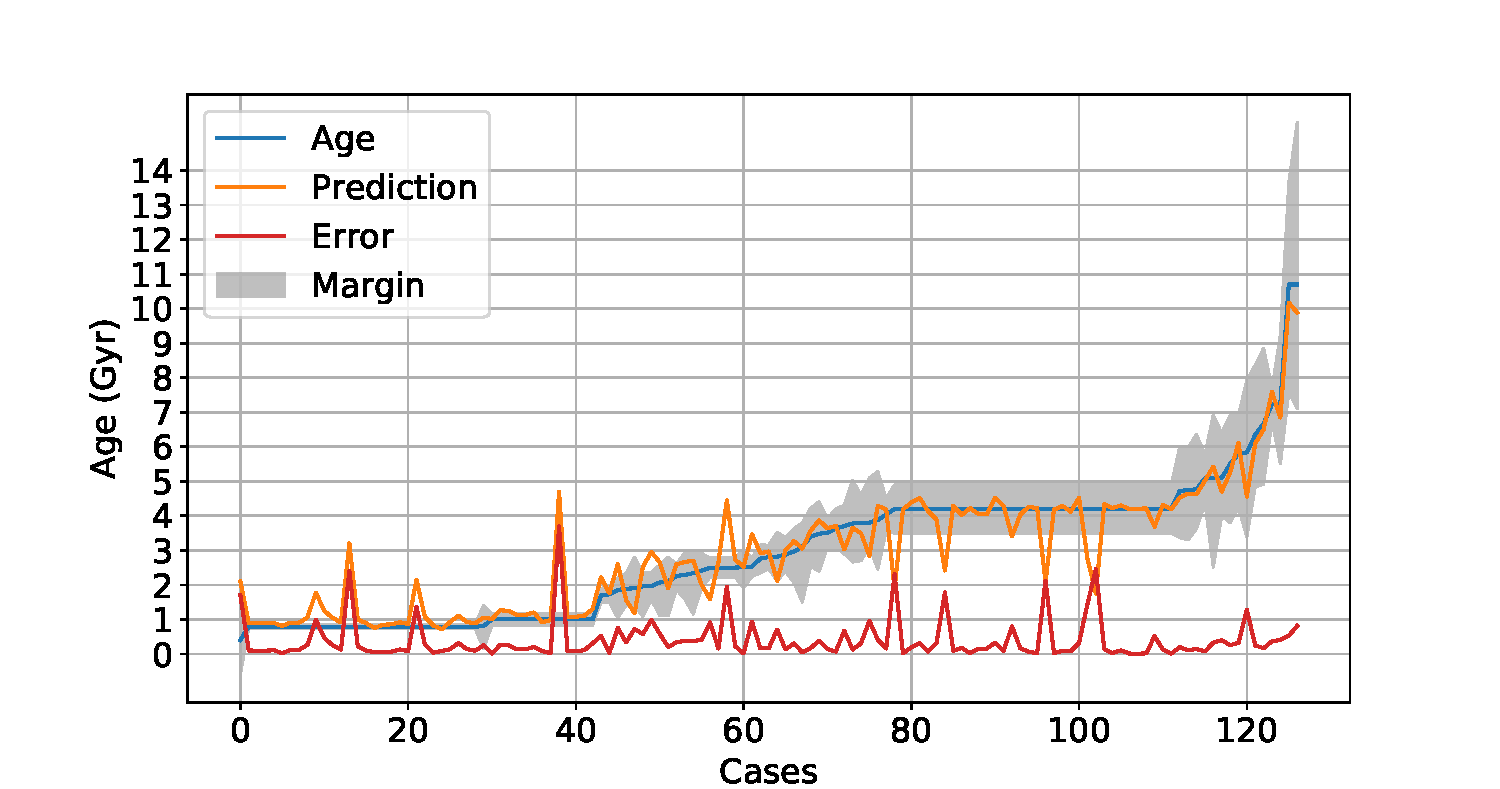
\includegraphics[width=0.8\linewidth]{Figuras/Experimentos/B_A_stacking_2.pdf}}
\end{center}
\caption{Predicción detallada para el modelo de stacking. Se observa la edad real (en azul), la predicción de los modelos (en naranja), y el error correspondiente (en rojo).}
 \label{fig:benchA_details_stacking}
\end{figure}

\begin{figure}[t]
\begin{center}
 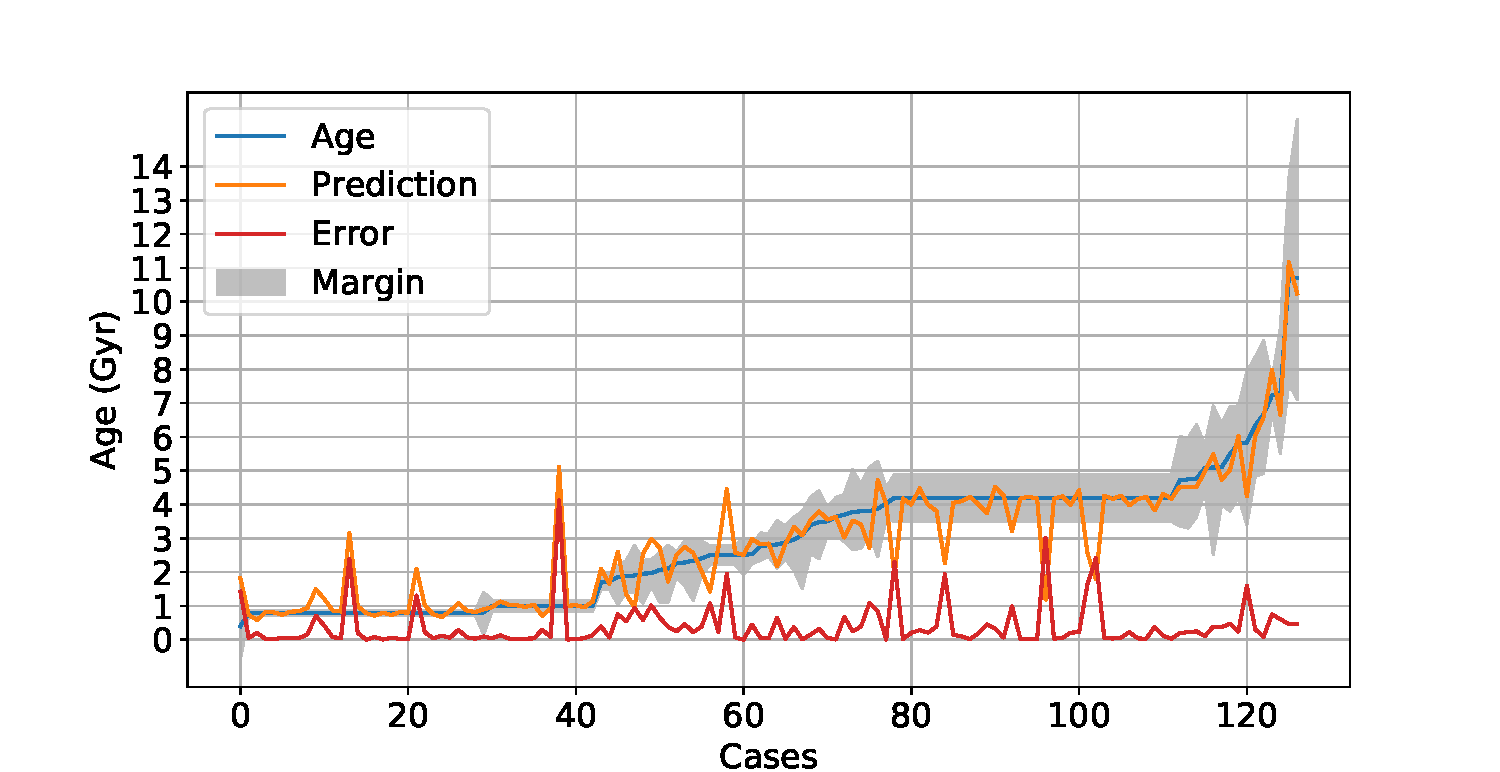
\includegraphics[width=0.8\linewidth]{Figuras/Experimentos/B_A_nnet_2.pdf}}
\end{center}
\caption{Predicción detallada para el modelo de la Red Neuronal. Se observa la edad real (en azul), la predicción de los modelos (en naranja), y el error correspondiente (en rojo).}
 \label{fig:benchA_details_nnet}
\end{figure}

\begin{figure}[t]
\begin{center}
 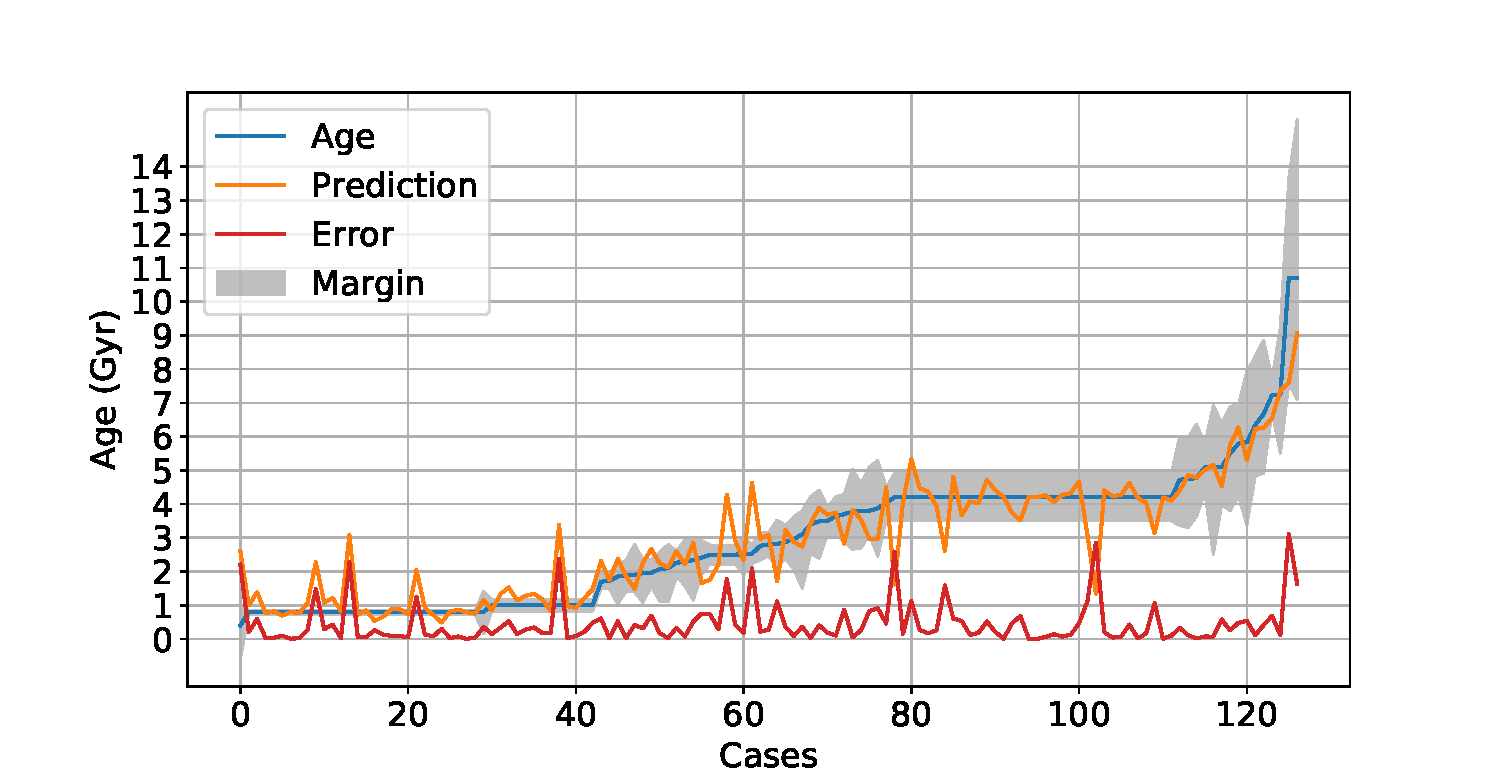
\includegraphics[width=0.8\linewidth]{Figuras/Experimentos/B_A_gp_2.pdf}}
\end{center}
\caption{Predicción detallada para el modelo de Gaussian Process. Se observa la edad real (en azul), la predicción de los modelos (en naranja), y el error correspondiente (en rojo).}
 \label{fig:benchA_details_gp}
\end{figure}

\begin{figure}[t]
\begin{center}
 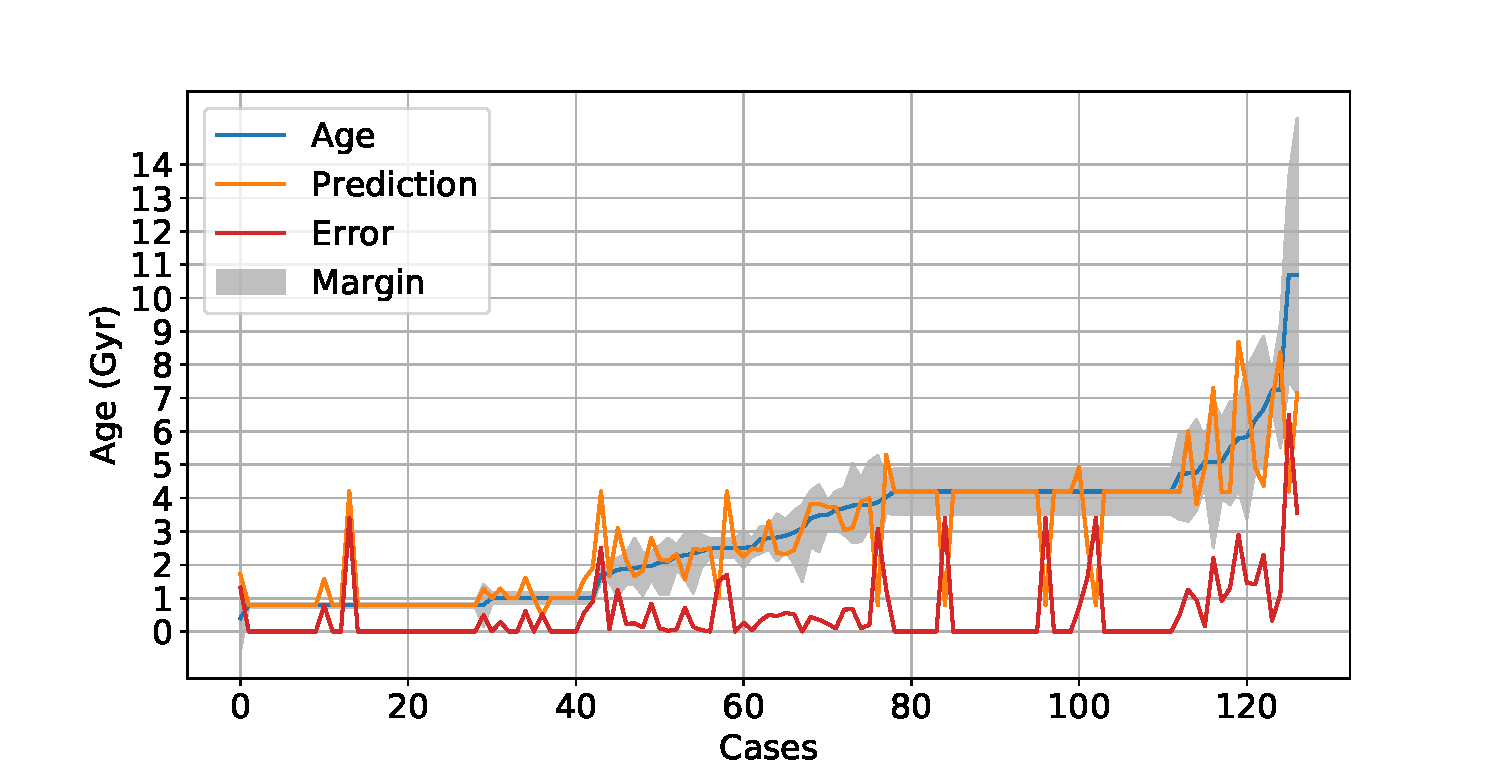
\includegraphics[width=0.8\linewidth]{Figuras/Experimentos/B_A_knn_2.pdf}}
\end{center}
\caption{Predicción detallada para el modelo de kNN. Se observa la edad real (en azul), la predicción de los modelos (en naranja), y el error correspondiente (en rojo).}
 \label{fig:benchA_details_knn}
\end{figure}

\begin{figure}[t]
\begin{center}
 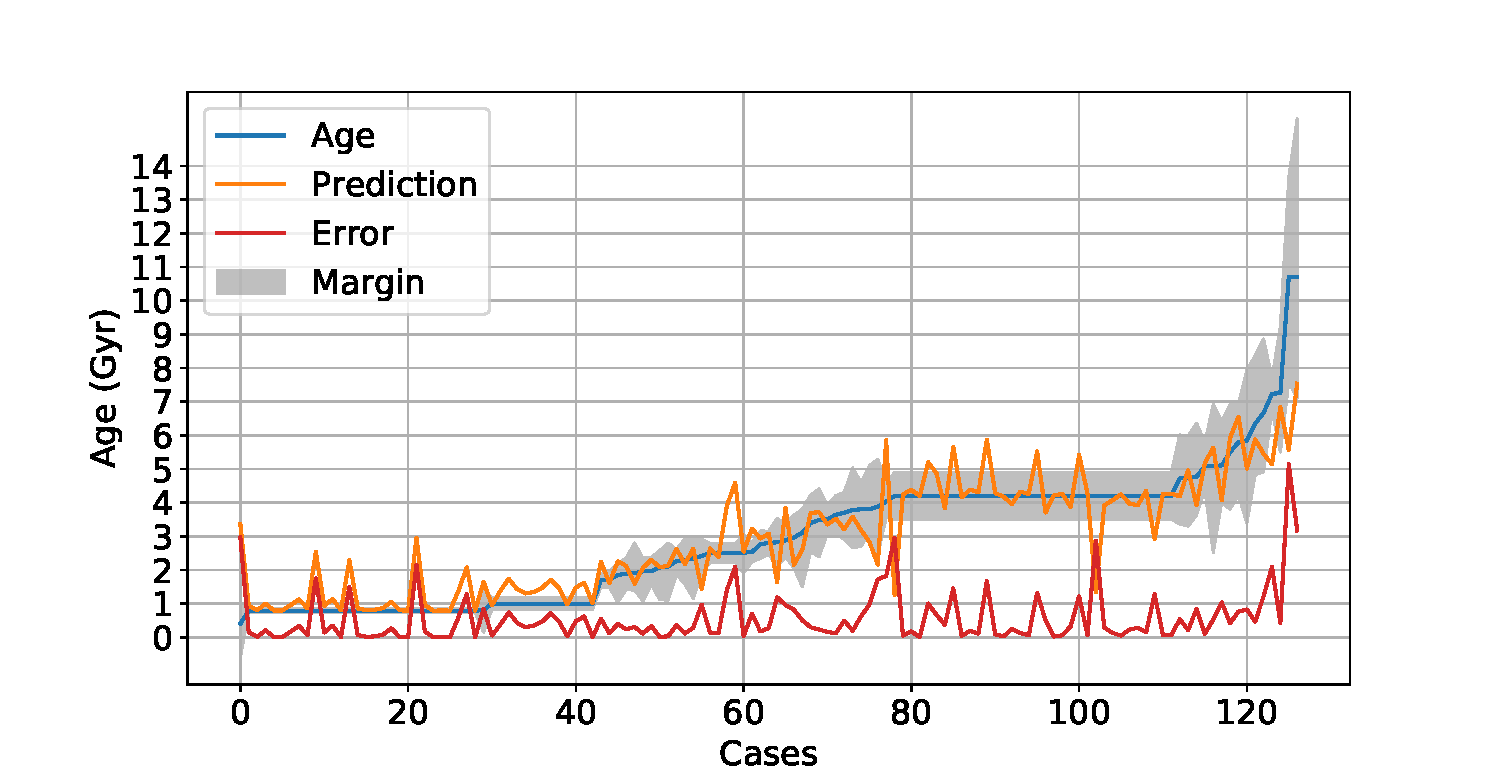
\includegraphics[width=0.8\linewidth]{Figuras/Experimentos/B_A_rf_2.pdf}}
\end{center}
\caption{Predicción detallada para el modelo de Random Forest. Se observa la edad real (en azul), la predicción de los modelos (en naranja), y el error correspondiente (en rojo).}
 \label{fig:benchA_details_rf}
\end{figure}

\begin{figure}[t]
\begin{center}
 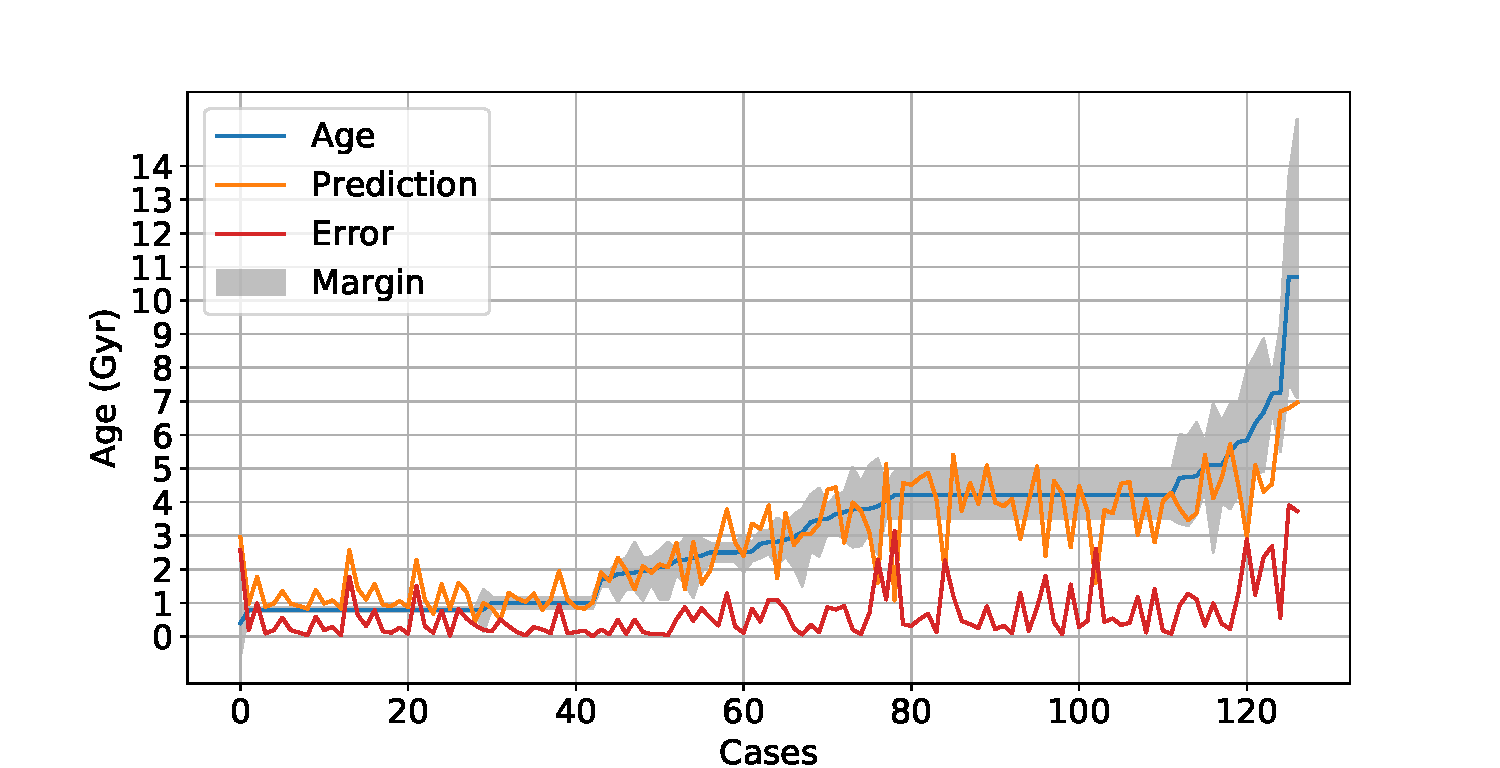
\includegraphics[width=0.8\linewidth]{Figuras/Experimentos/B_A_svm_2.pdf}}
\end{center}
\caption{Predicción detallada para el modelo de Support Vector Machine. Se observa la edad real (en azul), la predicción de los modelos (en naranja), y el error correspondiente (en rojo).}
 \label{fig:benchA_details_svm}
\end{figure}

\begin{figure}[t]
\begin{center}
 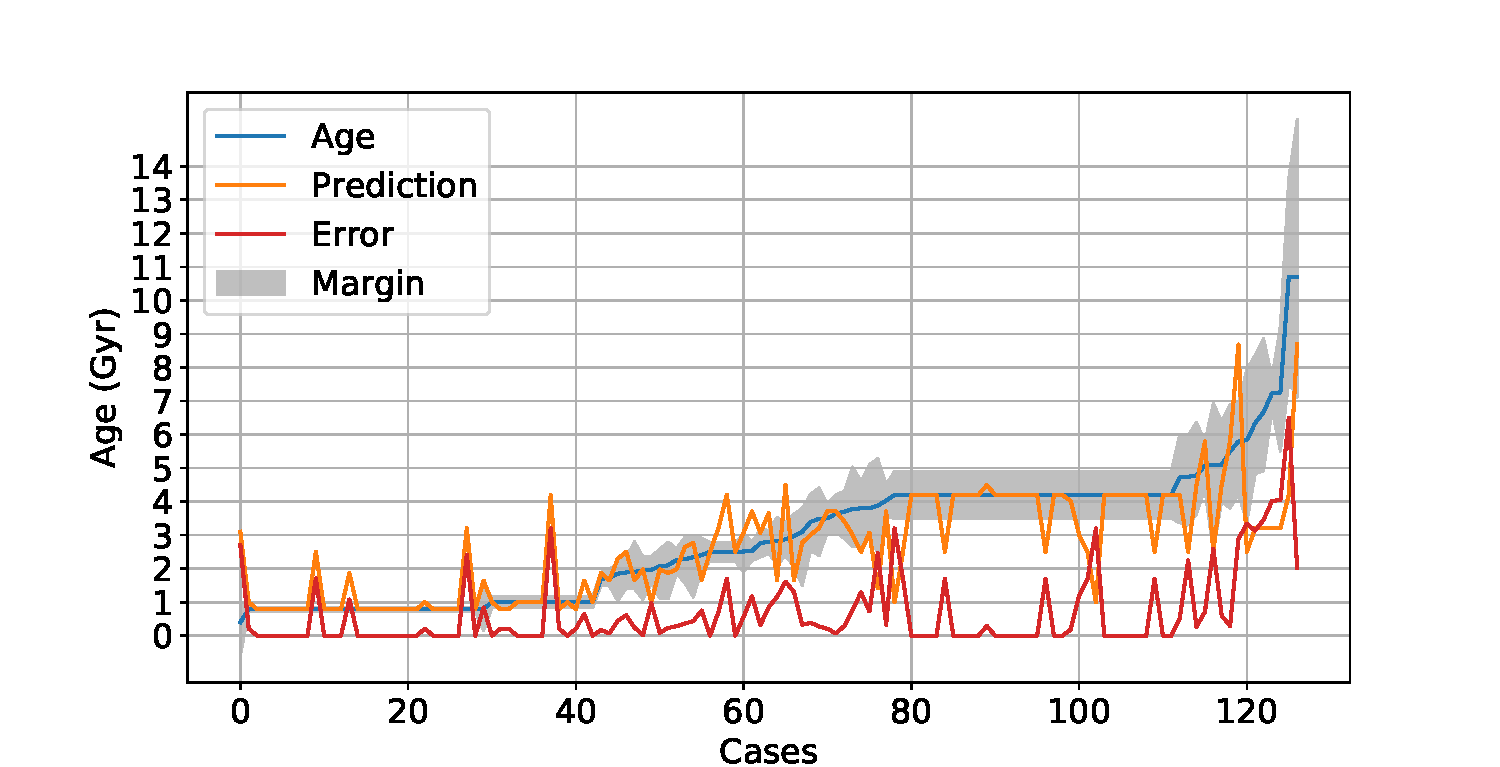
\includegraphics[width=0.8\linewidth]{Figuras/Experimentos/B_A_dtr_2.pdf}}
\end{center}
\caption{Predicción detallada para el modelo de Decision Tree. Se observa la edad real (en azul), la predicción de los modelos (en naranja), y el error correspondiente (en rojo).}
 \label{fig:benchA_details_dtr}
\end{figure}

\begin{figure}[t]
\begin{center}
 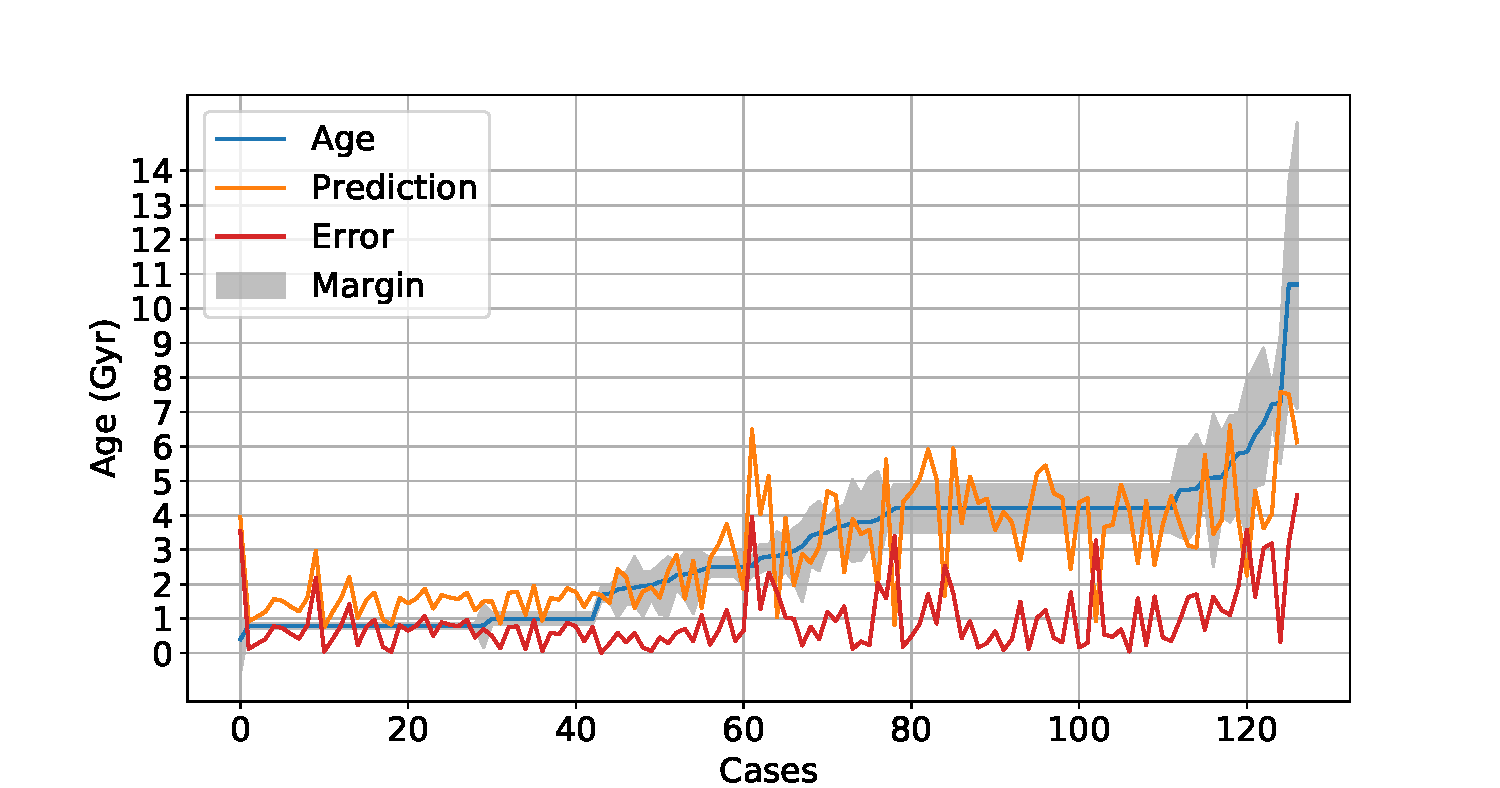
\includegraphics[width=0.8\linewidth]{Figuras/Experimentos/B_A_lr_2.pdf}}
\end{center}
\caption{Predicción detallada para el modelo de Linear Regressor. Se observa la edad real (en azul), la predicción de los modelos (en naranja), y el error correspondiente (en rojo).}
 \label{fig:benchA_details_lr}
\end{figure}

\begin{figure}[t]
\begin{center}
 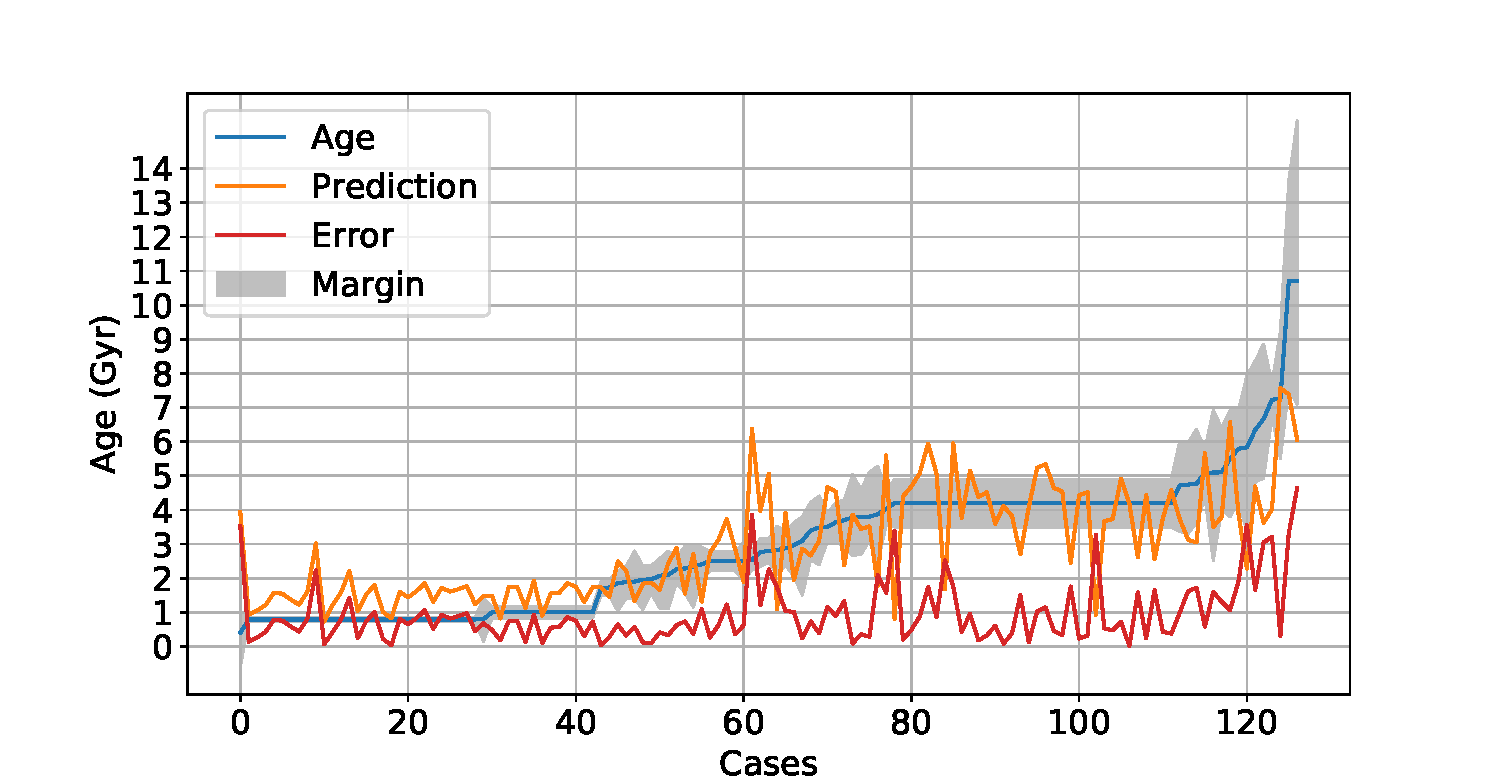
\includegraphics[width=0.8\linewidth]{Figuras/Experimentos/B_A_bayes_2.pdf}}
\end{center}
\caption{Predicción detallada para el modelo de Bayessian Regression. Se observa la edad real (en azul), la predicción de los modelos (en naranja), y el error correspondiente (en rojo).}
 \label{fig:benchA_details_bayes}
\end{figure}


\begin{table}
\centering
\scalebox{0.6}{
\begin{tabular}{l|ccccccccc}  
\toprule
Benchmark & nnet & lr & dtr & rf & svm & bayes & knn & gp & stacking \\
\midrule
\textbf{A}  & 73.23 & 35.43 & 63.78 & 60.63 & 46.46 & 32.28 & \textbf{77.95} & 62.20 & 62.99\\
\textbf{B1}  & \textbf{59.84} & 29.92 & 51.18 & 48.03 & 37.79 & 28.35 & 55.91 & 51.97 & n/a \\
\textbf{B2}  & 28.45 & 30.96 & 21.34 & 25.94 & \textbf{33.05} & 29.71 & 25.52 & 30.96 & n/a\\
\textbf{C}  & 34.37 & 21.87 & 9.37 & 21.87 & 12.50 & 21.87 & 15.62 & \textbf{40.62} & 34.37\\
\bottomrule
\end{tabular}
}%end of scalebox
\caption{Precisión de todos los métodos en los diferentes benchmarks. La precisión se mide como el porcentaje de estimaciones de edad que caen dentro del margen de confianza asociado a cada estrella.}\label{table:precisions}
\end{table}


\subsection{Benchmark B: Escenario de generalización}

Aquí se analiza la capacidad de generalización de todos los modelos para el problema de datación estelar. Las Figuras \ref{fig:benchB1} y \ref{fig:benchB2} muestran el rendimiento en los escenarios de evaluación B1 y B2, respectivamente.

Teniendo en cuenta que el Benchmark B1 se centra en analizar la precisión de los modelos estimando edades de estrellas más antiguas a las que han visto durante el entrenamiento. Obviamente, el error promedio de lo modelos ha aumentado. El mejor rendimiento se observa en la Red Neuronal, con un MAE de 1,47 Gyr. Las estimaciones detalladas se pueden ver en la Figura \ref{fig:benchB1_best}, donde se puede señalar cómo la Red Neuronal es capaz de generalizar hasta 6 Gyr, asignando estimaciones de edad que en su mayoría se encuentran dentro del margen de confianza. La Tabla \ref{table:precisions} confirma este hecho, donde la Red Neuronal también exhibe la precisión más alta para el Benchmark B1.


\begin{figure}[t]
\begin{center}
 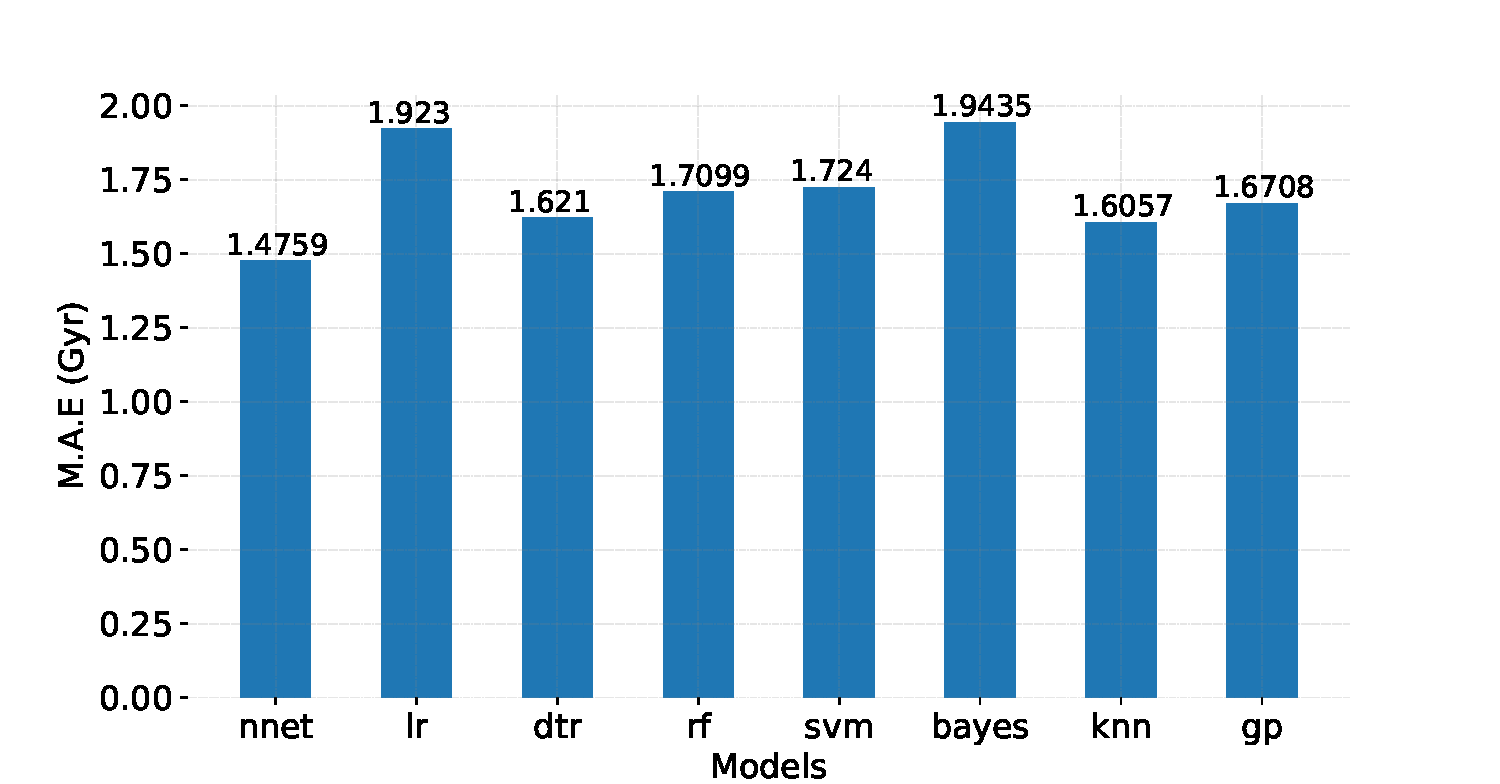
\includegraphics[width=0.8\linewidth]{Figuras/Experimentos/B_B1_models.pdf}}
\end{center}
\caption{Rendimiento de los modelos en función del MAE.}
 \label{fig:benchB1}
\end{figure}

\begin{figure}[t]
\begin{center}
 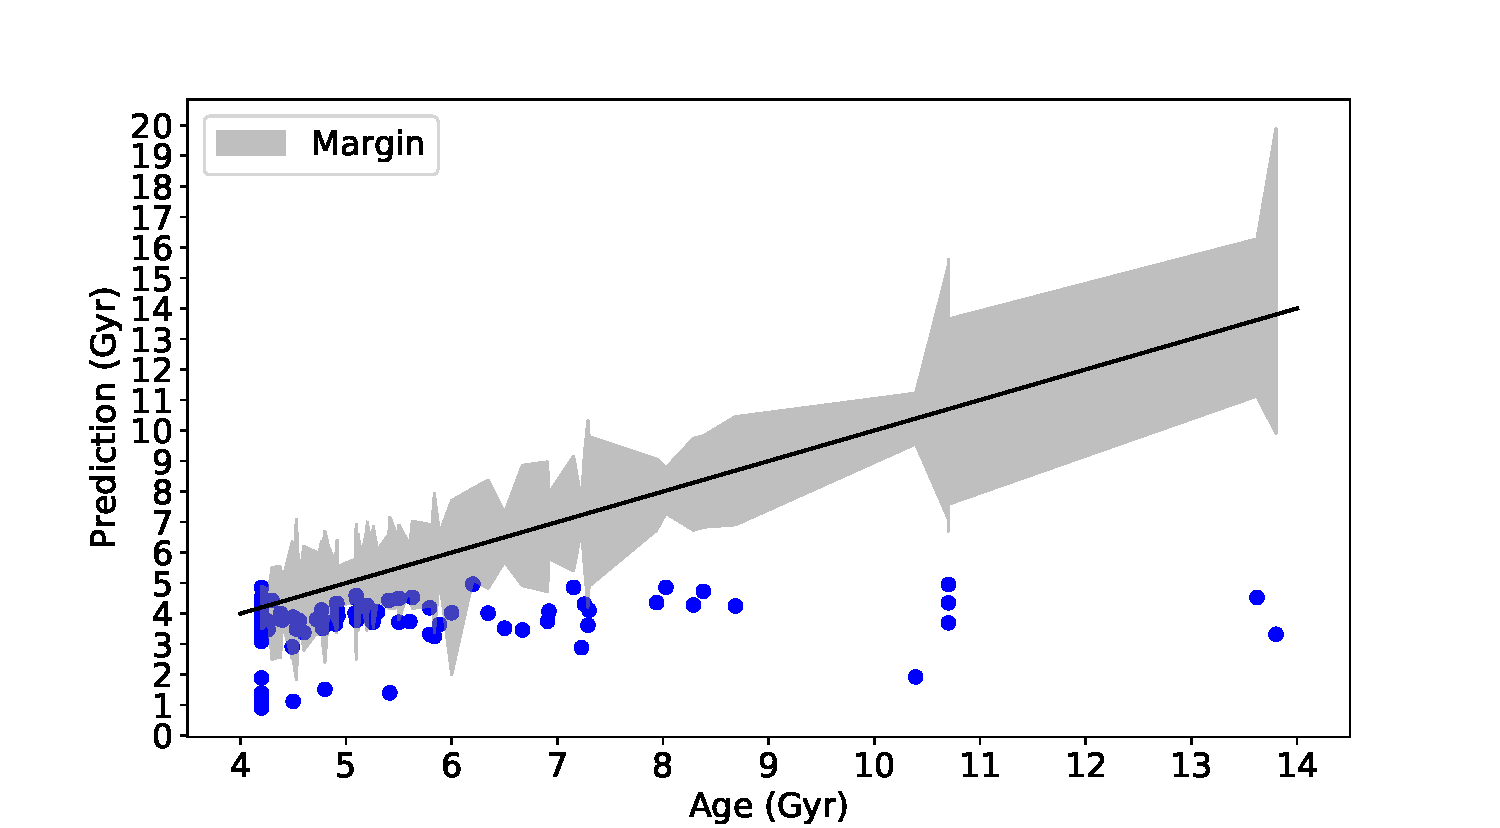
\includegraphics[width=0.8\linewidth]{Figuras/Experimentos/B_B1_nnet_1.pdf}}
\end{center}
\caption{Rendimiento para el mejor modelo del Benchmark B1: Red Neuronal.}
 \label{fig:benchB1_best}
\end{figure}


La historia es completamente diferente en el Benchmark B2. La Red Neuronal no es capaz de ser la mejor generalizando. Su error asciende hasta 1,85 Gyr, siendo superada por lr, rf, svm, knn, gp y bayes. Este último resulta ser el mejor modelo en este escenario, con un MAE de 1,48 Gyr. De la Figura \ref{fig:benchB2_best} se llega a la conclusión de que un regresor bayesiano es capaz de proporcionar edades precisas en el rango de 1 Gyr a 5 Gyr, es decir, el rango cubierto por la muestra de entrenamiento en este caso. En términos de precisión, la Tabla \ref{table:precisions} revela que svm para regresión es el modelo ganador, seguido de cerca por gp y lr. El modelo bayesiano, aunque tiene el MAE más bajo, presenta una precisión del 29.71 \%.

\begin{figure}[t]
\begin{center}
 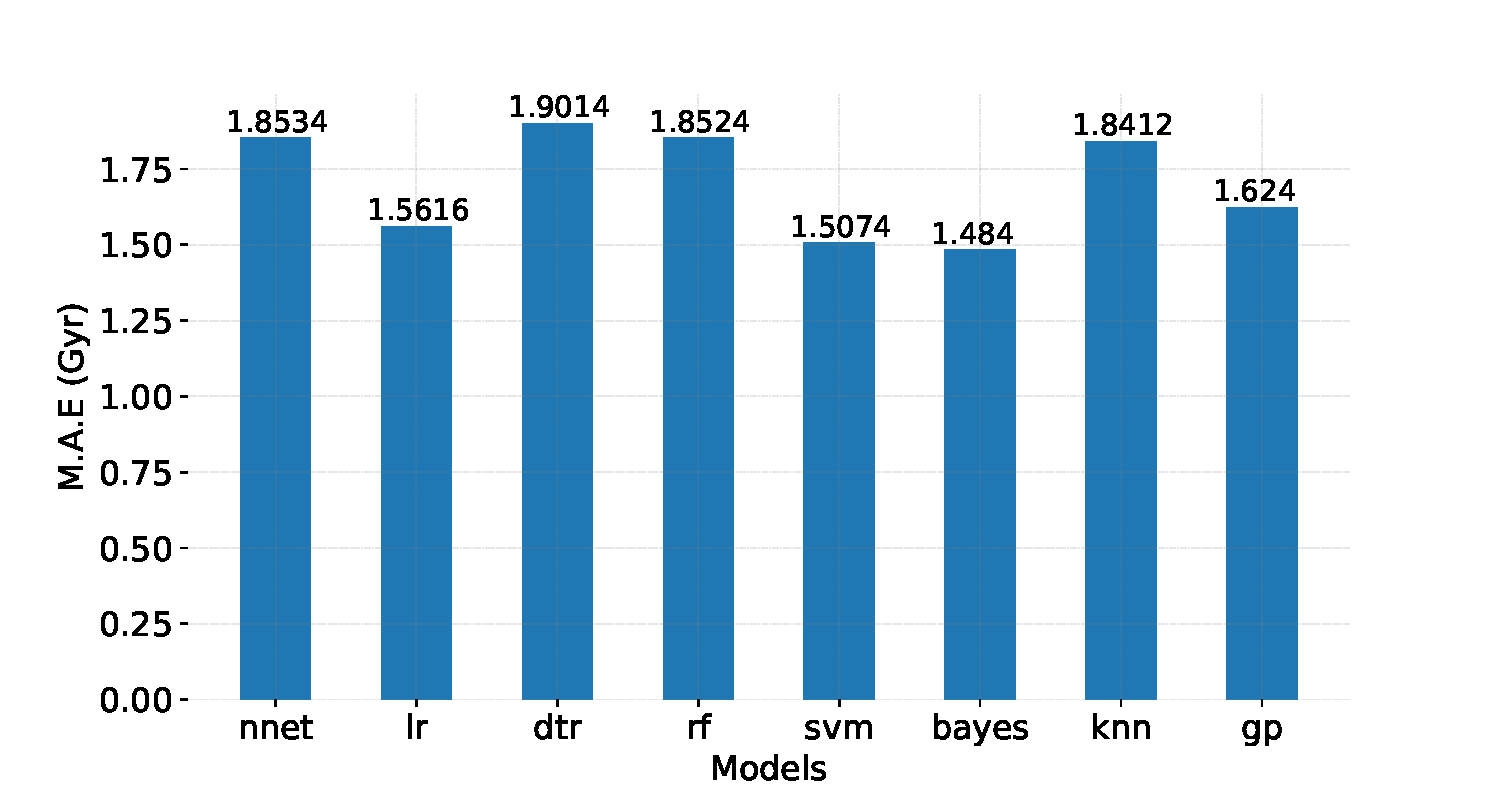
\includegraphics[width=0.8\linewidth]{Figuras/Experimentos/B_B2_models.pdf}}
\end{center}
\caption{Rendimiento de los modelos en función del MAE.}
 \label{fig:benchB2}
\end{figure}

\begin{figure}[t]
\begin{center}
 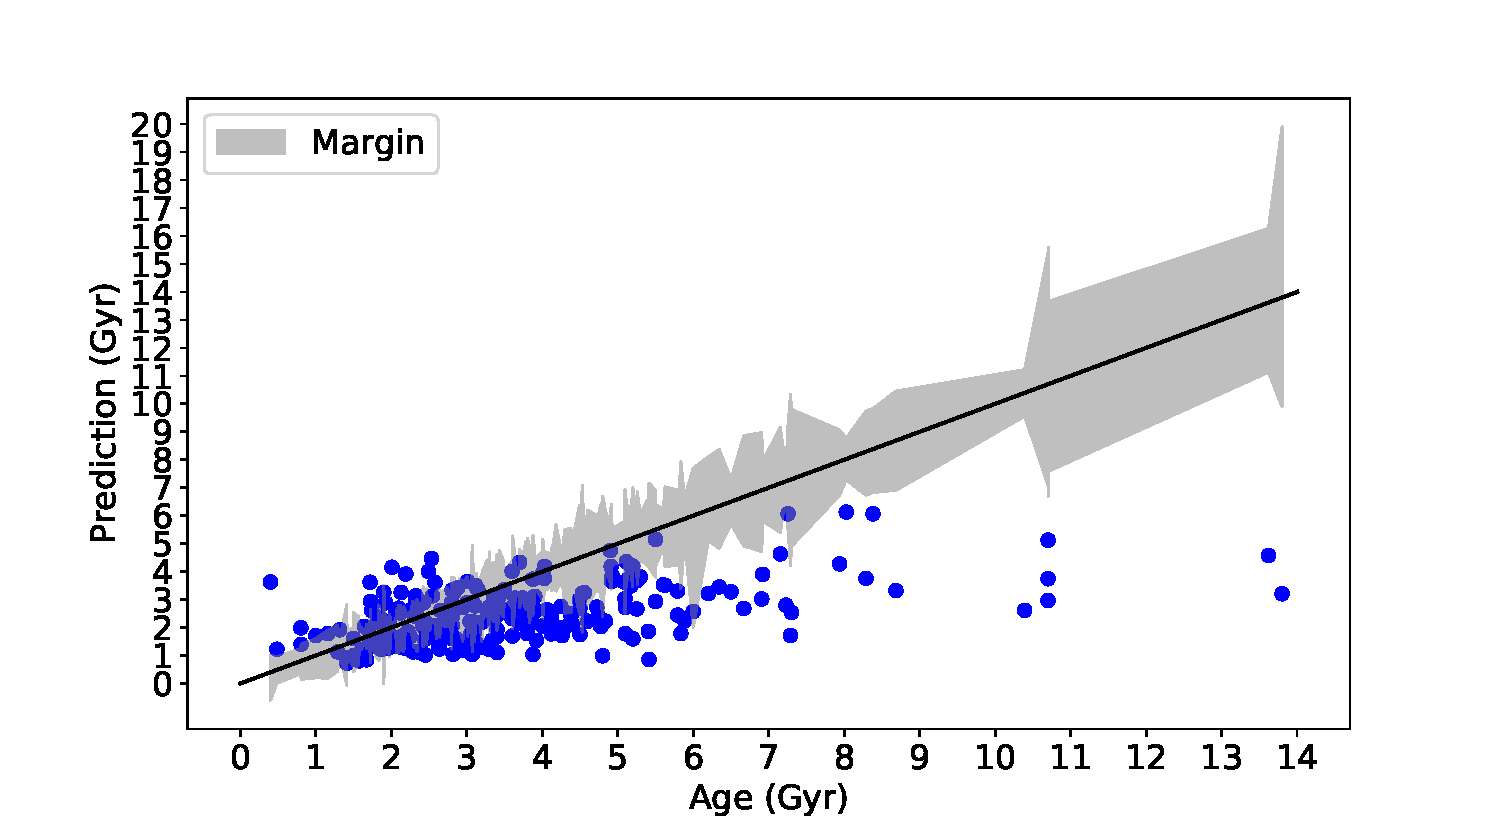
\includegraphics[width=0.8\linewidth]{Figuras/Experimentos/B_B2_bayes_1.pdf}}
\end{center}
\caption{Rendimiento para el mejor modelo del Benchmark B2: Bayessian Regression.}
 \label{fig:benchB2_best}
\end{figure}

Finalmente, en ambos escenarios se observa que todos los modelos tienden a subestimar las edades, aunque ese efecto es más pronunciado en el segundo Benchmark. Esto no es algo sorprendente, ya que en ambos casos las edades superiores a 4,2 Gyr no están cubiertas por las muestras de entrenamiento.


\subsection{Benchmark C: Rendimiento sobre la muestra de control}

Se mestra el MAE y la precisión para cada método para este Benchmark de control en la Figura \ref{fig:benchC} y en la Tabla \ref{table:precisions}, respectivamente. En esta ocasión, los tres mejores métodos son gp, nnet y su Stacking. Entre estos tres, descata el proceso gaussiano. En la Figura \ref{fig:benchC_best} se pueden inspeccionar las predicciones de las edades estelares usando este método frente a las edades de referencia para las estrellas de ese set. gp es el modelo con mayor precisión: $40.62\%$ de las predicciones caen dentro del margen de confianza del conjunto de datos. Para el Sol, gp predice una edad de 3,88 frente a una edad aceptada de 4,6 Gyr, subestimándola. De hecho, el modelo tiende a subestimar ligeramente la mayoría de las edades. Se observa este comportamiento en todos lo modelos salvo en kNN y dtr. 

\begin{figure}[t]
\begin{center}
 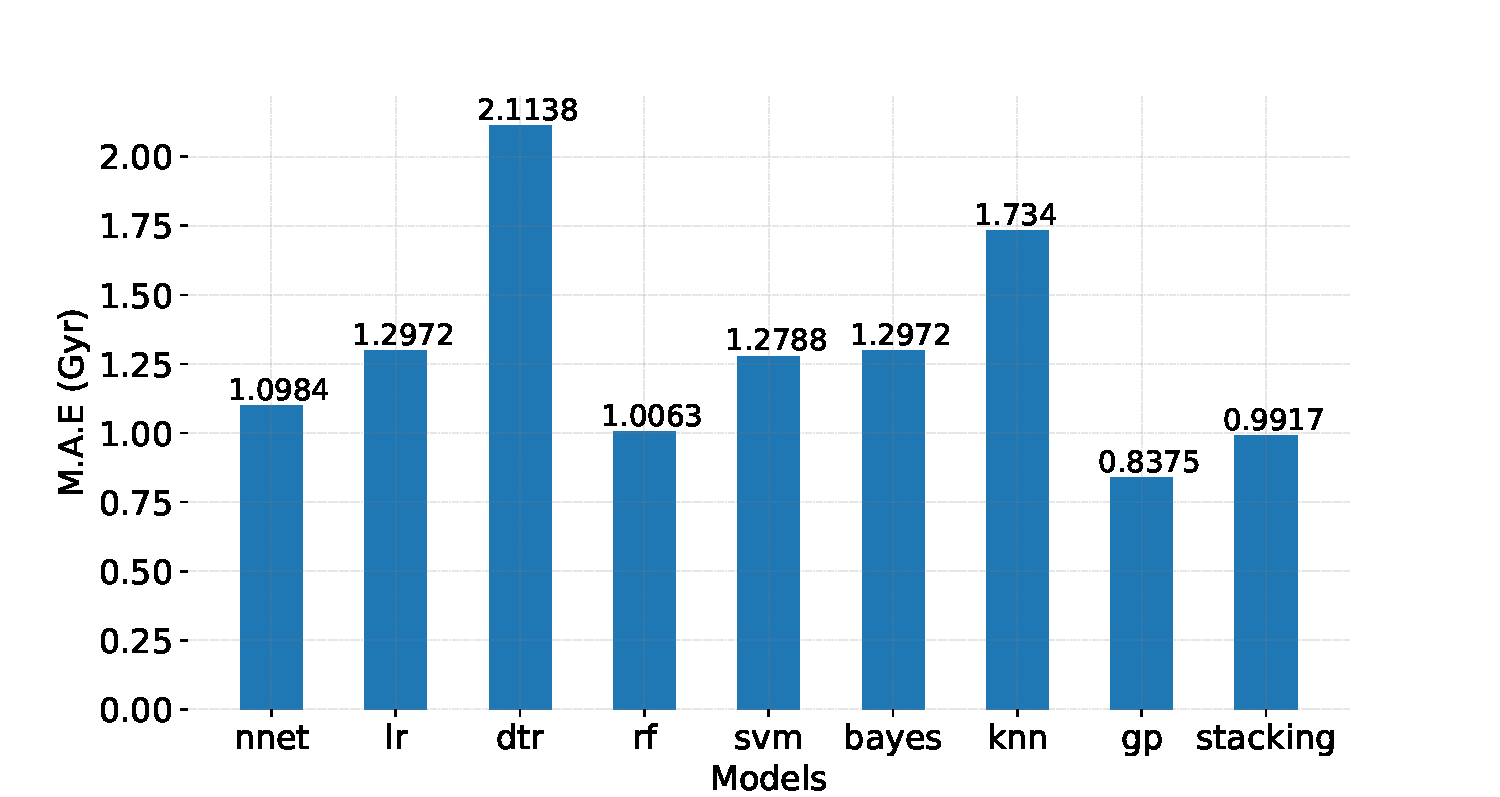
\includegraphics[width=0.8\linewidth]{Figuras/Experimentos/B_C_models.pdf}}
\end{center}
\caption{Rendimiento de los modelos en función del MAE.}
 \label{fig:benchC}
\end{figure}

\begin{figure}[t]
\begin{center}
 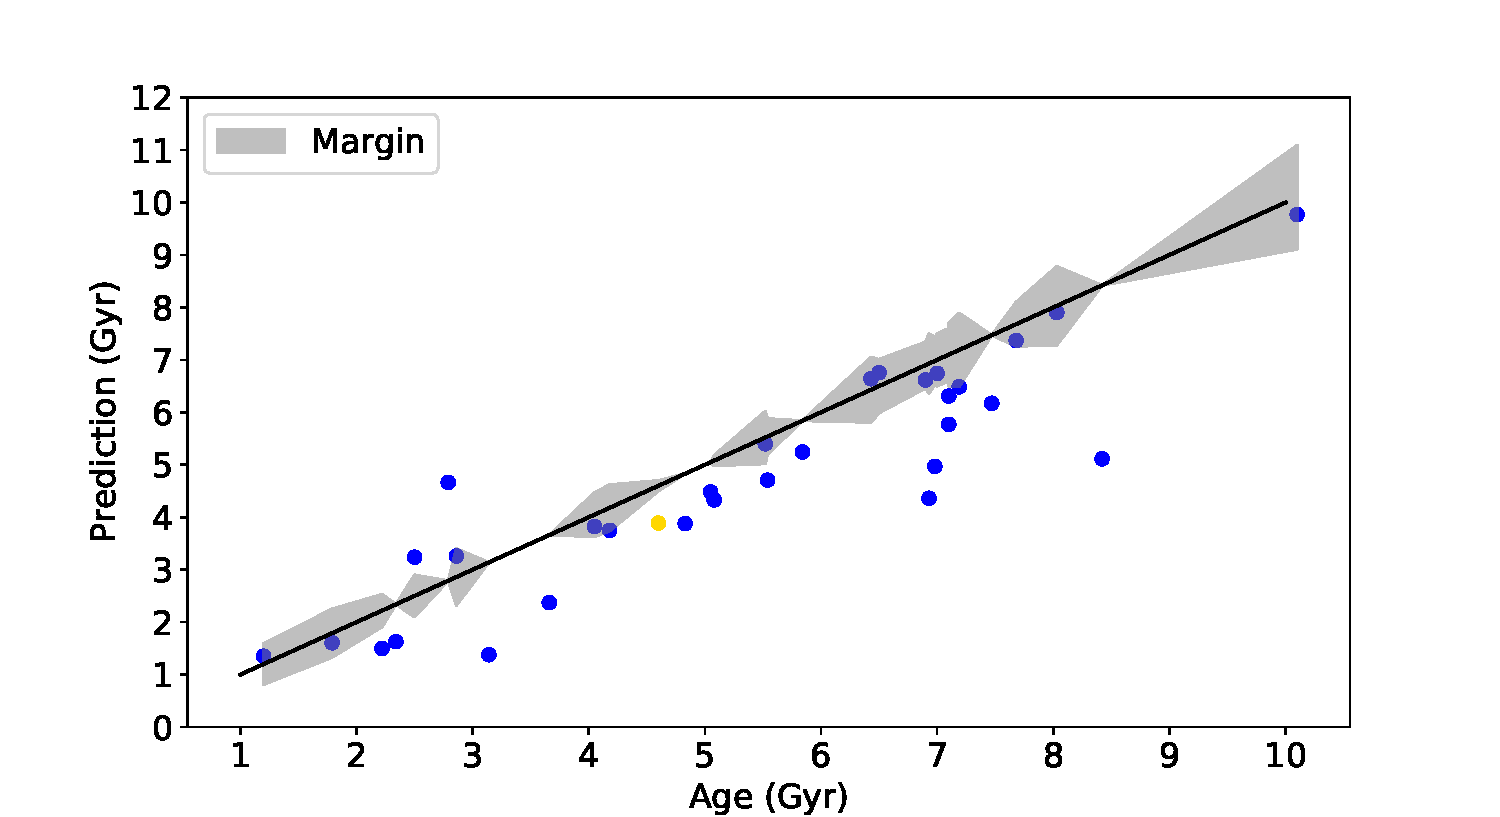
\includegraphics[width=0.8\linewidth]{Figuras/Experimentos/B_C_gp_1.pdf}}
\end{center}
\caption{Rendimiento para el mejor modelo del Benchmark B2: Gaussian Process. El punto amarillo se corresponde con la representación de la estimación de la edad del Sol.}
 \label{fig:benchC_best}
\end{figure}

%Precision for the SUN
Respecto a la precisión en las estimaciones para la edad del Sol, 4,6 Gyr, se proporciona en la Tabla \ref{table:sun_results} la edad específica obtenida en cada uno de los modelos. Todos los métodos subestiman, y rf obtiene la predicción más cercana, seguido de dtr y kNN.


\begin{table}
\centering
\scalebox{0.6}{
\begin{tabular}{l|ccccccccc}  
\toprule
\textbf{Métodos}  & nnet & lr & dtr & rf & svm & bayes & knn & gp & stacking \\
\midrule
Sol (4.6 Gyr)  & 4.02 & 3.92 & 4.49 & 4.76 & 3.81 & 3.91 & 4.49 & 3.88 & 4.02\\
\bottomrule
\end{tabular}
}%end of scalebox
\caption{Edad estimada para el Sol en Gyr. El método más preciso es rf. }\label{table:sun_results}
\end{table}

Comparando los resultados de los Benchmark A (Figura \ref{fig:benchA_models}) y C (Figura \ref{fig:benchC}), se puede concluir que: a) los modelos ganadores son comunes (nnet, gp y stacking); b) kNN y dtr sufren una degración considerable de su rendimiento, ya que dependen en gran medida de la distribución de datos utilizada durante su entrenamiento; y c) bayes y lr son similares, mostrando un incremento similar en sus correspondientes MAEs, pero al mismo tiempo ofreciendo cierta estabilidad entre escenarios.


\chapter{Continual learning} 

\chapter{Conclusiones}

Se ha presentado un análisis exhaustivo comparando el estado del arte de modelos de regresión de IA, entrenados y probados para la datación estelar usando girocronología. Con base en este estudio, se informa de los siguientes hallazgos sobre el rendimiento y la capacidad de generalización de los modelos de regresión para la estimación de edades estelares.

En primer lugar, ¿existe un modelo ganador? El estudio demuestra que un modelo de datación estelar basado en una Red Neuronal como la desarrollada en este proyecto, proporciona resultados notables en términos de compensación entre generalización y precisión. Los experimentos revelan que el rendimiento del modelo nnet es bueno en los Benchmark A y C, pero también en B1, donde tiene que generalizarse a edades desconocidas. Es un modelo simple, un MLP con 3 capas ocultas, que podría extenderse (\eg Usando capas 1D CNN) posiblemente ofreciendo mejores resultados. Se deja la puerta abierta para futuras investigaciones. Si los profesionales buscan la solución con el menor error, el mensaje es: debe utilizarse un modelo de stacking que combine procesos gaussianos y redes neuronales. Finalmente, se recomienda una regresión bayesiana si los datos de entrenamiento disponibles pertenecen principalmentea clústeres de estrellas. En segundo lugar, \emph{todos} los modelos tienden a subestimar en general, y no solo en el Benchmark B1, donde sería natural. Por tanto, se cree ve una interesante línea de trabajo futuro en reducir este sesgo. Y tercero, el estudio revela resultados promeedores para el problema de datación estelar. Un error de $<0.5$ Gyr se puede considerar como un gran avance en el campo.

